\documentclass{article} % for initial submission
\usepackage[a4paper, total={6in, 8in}]{geometry}
% \documentclass[accepted]{uai2023} % after acceptance, for a revised
                                    % version; also before submission to
                                    % see how the non-anonymous paper
                                    % would look like

%% There is a class option to choose the math font
% \documentclass[mathfont=ptmx]{uai2023} % ptmx math instead of Computer
% Modern (has noticable issues)
% \documentclass[mathfont=newtx]{uai2023} % newtx fonts (improves upon
 % ptmx; less tested, no support)
% NOTE: Only keep *one* line above as appropriate, as it will be replaced
%       automatically for papers to be published. Do not make any other
%       change above this note for an accepted version.

%% Choose your variant of English; be consistent
\usepackage[american]{babel}
% \usepackage[british]{babel}

\usepackage{amsfonts}
\newcommand{\argmin}{arg\,min}
\usepackage{subcaption}
\usepackage{algorithm}
\usepackage{algpseudocode}
\renewcommand{\algorithmicrequire}{\textbf{Input:}}
\renewcommand{\algorithmicensure}{\textbf{Output:}}
\usepackage{bbm}
\usepackage{graphicx}
\graphicspath{ {./../code/} }

\newtheorem{theorem}{Theorem}[section]
\newtheorem{corollary}{Corollary}[theorem]
\newtheorem{lemma}[theorem]{Lemma}

\newtheorem{innercustomthm}{Theorem}
\newenvironment{customthm}[1]
  {\renewcommand\theinnercustomthm{#1}\innercustomthm}
  {\endinnercustomthm}


\newcommand{\dfdx}{\frac{\partial f}{\partial x_s}}
\newcommand{\xc}{\mathbf{x_c}}
\newcommand{\DY}{\mathbf{\Delta Y}}
\newcommand{\xb}{\mathbf{x}}
\newcommand{\Xcb}{\mathcal{X}_c}
\newcommand{\Xb}{\mathcal{X}}


%% Some suggested packages, as needed:
\usepackage{natbib} % has a nice set of citation styles and commands
    \bibliographystyle{plainnat}
    \renewcommand{\bibsection}{\subsubsection*{References}}
\usepackage{mathtools} % amsmath with fixes and additions
% \usepackage{siunitx} % for proper typesetting of numbers and units
\usepackage{booktabs} % commands to create good-looking tables
\usepackage{tikz} % nice language for creating drawings and diagrams

% for cross referencing the main text
% PLEASE ONLY USE xr IN THE SUPPLEMENTARY MATERIAL. 
% In the main paper, hard code any cross-reference to the supplementary material. 
\usepackage{xr} 
\externaldocument{uai-paper}

%% Provided macros
% \smaller: Because the class footnote size is essentially LaTeX's \small,
%           redefining \footnotesize, we provide the original \footnotesize
%           using this macro.
%           (Use only sparingly, e.g., in drawings, as it is quite small.)

%% Self-defined macros
\newcommand{\swap}[3][-]{#3#1#2} % just an example

\title{RHALE: Robust and Heterogeneity-aware Accumulated Local Effects\\(Supplementary Material)}

% The standard author block has changed for UAI 2023 to provide
% more space for long author lists and allow for complex affiliations
%
% All author information is authomatically removed by the class for the
% anonymous submission version of your paper, so you can already add your
% information below.
%
% Add authors
% \author[1]{\href{mailto:<jj@example.edu>?Subject=Your UAI 2023 paper}{Jane~J.~von~O'L\'opez}{}}
% \author[1]{Harry~Q.~Bovik}
% \author[1,2]{Further~Coauthor}
% \author[3]{Further~Coauthor}
% \author[1]{Further~Coauthor}
% \author[3]{Further~Coauthor}
% \author[3,1]{Further~Coauthor}
% % Add affiliations after the authors
% \affil[1]{%
%     Computer Science Dept.\\
%     Cranberry University\\
%     Pittsburgh, Pennsylvania, USA
% }
% \affil[2]{%
%     Second Affiliation\\
%     Address\\
%     …
% }
% \affil[3]{%
%     Another Affiliation\\
%     Address\\
%     …
%   }

\begin{document}

\maketitle

%This Supplementary Material should be submitted as a separate file. Please do not append the Supplementary Material to the main paper.

%Fig. \ref{fig:pitt} and Eq \ref{eq:example} in the main paper can be cross referenced using \texttt{xr}.

\appendix

\section{Theoretical Evidence}

In this Section, we provide proofs for the equations used in the main paper.

\subsection{Proof that \(\hat{\mu}(z_1, z_2)\) is an unbiased estimator of \( \mu(z_1, z_2)\)}
\label{sec:proof-1}

This proof is required for Theorem 1 (Section~\ref{sec:proof-2}).
We want to show that

\[\hat{\mu}(z_1, z_2) = \frac{1}{|\mathcal{S}|} \sum_{i: \mathbf{x}^i
  \in \mathcal{S}} f^s(\mathbf{x}^i) \]
%
is an unbiased estimator of:
%
\[\mu(z_1, z_2) = \frac{\int_{z_1}^{z_2} \mathbb{E}_{X_c|z} \left [
      f^s(z, X_c) \right ] \partial z}{z_2 - z_1} \]
%
under the assumptions that
(a) \(z\) follows a uniform distribution in
\([z_1, z_2]\), i.e., \(z \sim \mathcal{U}(z_1, z_2)\),
(b) \(\tilde{X}\) is a random variable with PDF
\(p(\tilde{\xb}) = p(\xc|z)p(z) = \frac{1}{z_2-z_1}p(\xc|z) \) and
(c) the points \(\mathbf{x}^i\) are i.i.d. samples from
\(p(\tilde{\xb})\).
We want to show that \(\mathbb{E}_{\tilde{X}} [\hat{\mu}(z_1, z_2)] = \mu(z_1, z_1)\).

\paragraph{Proof Description}
We show that (a) \(\mu(z_1, z_2) = \mathbb{E}_{\tilde{X}} [f^s(\tilde{X})]\) and
we use the fact that
(b) the population mean is an unbiased estimator of the expected value.

\paragraph{Proof}
\begin{align}
  \mu(z_1, z_2)
  = \frac{\int_{z_1}^{z_2} \mathbb{E}_{X_c|z} [f^s(z, X_c)] \partial z}{z_2 - z_1}
  = \mathbb{E}_{z \sim \mathcal{U}(z_1, z_2)}[\mathbb{E}_{X_c|z} [f^s(z, X_c)]]
  = \mathbb{E}_{\tilde{X}} [f^s(\tilde{X})]
  = \mathbb{E}_{\tilde{X}} [\hat{\mu}(z_1, z_2)]
\end{align}

\subsection{Proof that \(\hat{\sigma}^2(z_1, z_2)\) is an unbiased estimator of \(\sigma_*^2(z_1, z_2)\)}
\label{sec:proof-2}

This equation is used in Section 3.1 of the main paper.
We want to show that

\[\hat{\sigma}^2(z_1, z_2) = \frac{1}{|\mathcal{S}_k - 1|}
\sum_{i:\mathbf{x}^i \in \mathcal{S}_k} \left ( f^s(\mathbf{x}^i) -
  \hat{\mu}(z_1, z_2) \right )^2\]
%
is an unbiased estimator of

\[\sigma^2_*(z_1, z_2) = \frac{\int_{z_1}^{z_2} \mathbb{E}_{X_c|X_s=z}
  \left [ (f^s(z, X_c) - \mu(z_1, z_2) )^2 \right] \partial z}{z_2 -
  z_1} \]
%
under the assumptions that (a) \(z\) follows a uniform distribution
in \([z_1, z_2]\), i.e., \(z \sim \mathcal{U}(z_1, z_2)\), (b)
\(\tilde{X}\) is a random variable with PDF
\(p(\tilde{\xb}) = p(\xc|z)p(z) = \frac{1}{z_2-z_1}p(\xc|z) \) and (c)
the points \(\mathbf{x}\) are i.i.d. samples from
\(p(\tilde{\xb})\). We want to show that
\(\mathbb{E}_{\tilde{X}} [\hat{\sigma}^2(z_1, z_2)] = \sigma_*^2(z_1, z_1)\).

\paragraph{Proof Description}

We show (a) that
\(\sigma^2_*(z_1, z_2) = \mathbb{E}_{\tilde{X}} \left [ (f^s(\tilde{X}) - \mathbb{E}_{\tilde{X}}[\hat{\mu}(z_1, z_2)] )^2 \right]\) and
then (b) we use the fact that the sample variance is an unbiased
estimator of the distribution variance.

\paragraph{Proof}


\begin{align}
  \sigma^2_*(z_1, z_2) & = \frac{\int_{z_1}^{z_2} \mathbb{E}_{X_c|z}
                         \left [ (f^s(z, X_c) - \mu(z_1, z_2) )^2 \right] \partial z}{z_2 -
                         z_1} \\
                       & = \mathbb{E}_{z \sim \mathcal{U}(z_1, z_2)}\mathbb{E}_{X_c|z}
                         \left [ (f^s(z, X_c) - \mu(z_1, z_2) )^2 \right] \\
                       & = \mathbb{E}_{\tilde{X}} \left [ (f^s(\tilde{X}) - \mu(z_1, z_2) )^2 \right]\\
                       & = \mathbb{E}_{\tilde{X}} \left [ (f^s(\tilde{X}) - \mathbb{E}_{\tilde{X}}[\hat{\mu}(z_1, z_2)] )^2 \right]\\
                       & = \mathbb{E}_{\tilde{X}} \left [ \hat{\sigma}^2(z_1, z_2)  \right]
  \end{align}


\subsection{Proof Of Theorem 1}
\label{sec:proof-3}

\begin{customthm}{3.1}
  \label{sec:theorem-1-app}
  If we define (a) the residual \(\rho(z)\) as the difference between
  the expected effect at \(z\) and the bin effect, i.e,
  \(\rho(z) = \mu(z) - \mu(z_1, z_2)\), and (b)
  \(\mathcal{E}(z_1, z_2)\) as the mean squared residual of the bin,
  i.e.,
  \(\mathcal{E}(z_1, z_2) = \frac{\int_{z_1}^{z_2}\rho^2(z) \partial
    z}{z_2 - z_1}\), then it holds
%
\begin{equation}
    \label{eq:bin-uncertainty-proof}
 \sigma_*^2(z_1, z_2) = \sigma^2(z_1, z_2) + \mathcal{E}^2(z_1, z_2)
\end{equation}
\end{customthm}
%
We want to show that
\(\sigma_*^2(z_1, z_2) = \sigma^2(z_1, z_2) + \mathcal{E}^2(z_1,
z_2)\), where (a) the bin-error \(\mathcal{E}^2(z_1, z_2)\) is the
mean squared residual of the bin, i.e.
\(\mathcal{E}^2(z_1, z_2) = \frac{\int_{z_1}^{z_2}\rho^2(z) \partial
  z}{z_2 - z_1}\) and (b) the residual \(\rho(z)\) is the difference
between the expected effect at \(z\) and the bin effect, i.e
\(\rho(z) = \mu(z) - \mu(z_1, z_2)\).

\paragraph{Proof Description}

We use that \(\forall z \in [z_1, z_2]\), it holds that \(\mu(z_1, z_2) = \mu(z) - \rho(z)\) and then we split the terms appropriately to complete the proof.

\paragraph{Proof}

\begin{align}
  \sigma_*^2(z_1, z_2) &= \frac{1}{z_2 - z_1}\int_{z_1}^{z_2} \mathbb{E}_{X_c|z} \left [ \left( f^s( z, X_c) - \mu(z_1, z_2) \right)^2 \right] \partial z \\
                       &= \frac{1}{z_2 - z_1} \int_{z_1}^{z_2} \mathbb{E}_{X_c|z} \left [ \left ( f^s(z, X_c) - \mu(z) + \rho(z) \right )^2 \right] \partial z \\
                       &= \frac{1}{z_2 - z_1} \int_{z_1}^{z_2} \mathbb{E}_{X_c|z} \left [ (f^s(z, X_c) - \mu(z) )^2 + \rho(z)^2 + 2(f^s(z, X_c) -\mu(z))\rho(z) \right ] \partial z \\
                       &= \frac{1}{z_2 - z_1} \int_{z_1}^{z_2} \left (
                         \underbrace{\mathbb{E}_{X_c|z} \left [ (f^s(z, X_c) - \mu(z) )^2 \right ]}_{\sigma^2(z)}  +
                         \underbrace{\mathbb{E}_{X_c|z} \left [ \rho^2(z) \right]}_{\rho^2(z)} +
                         2 (\underbrace{\mathbb{E}_{X_c|z} \left [ (f^s(z, X_c)   \right ]}_{\mu(z)} - \mu(z)) \rho(z) )\right )  \partial z \\
                       &= \underbrace{\frac{1}{z_2 - z_1} \int_{z_1}^{z_2} \sigma^2(z) \partial z}_{\sigma^2(z_1, z_2)} + \underbrace{\frac{1}{z_2 - z_1} \int_{z_1}^{z_2} \rho^2(z) \partial z}_{\mathcal{E}^2(z_1, z_2)}\\
                       &= \sigma^2(z_1, z_2) + \mathcal{E}^2(z_1, z_2)
\end{align}

\subsection{Proof Of Corollary 2}


We want to show that, \textit{if a bin-splitting \(\mathcal{Z}\) minimizes the accumulated error, then it also minimizes
  \(\sum_{k=1}^K\sigma_*^2(z_1, z_2) \Delta z_k \)}.
In mathematical terms, we want to show that:

\[ \mathcal{Z}^* = \argmin_{\mathcal{Z}} \sum_{k=1}^K \sigma_*^2(z_{k-1}, z_k) \Delta z_k \Leftrightarrow \mathcal{Z}^* = \argmin_{\mathcal{Z}} \sum_{k=1}^K \mathcal{E}^2(z_{k-1}, z_k) \Delta z_k \]

\paragraph{Proof Description}

The key-point for the proof is that the term \(\sum_{k=1}^K \sigma^2(z_{k-1}, z_k) \Delta z_k \) is
independent of the bin partitioning \(\mathcal{Z}\). In Eq.(16) we use Eq.8 of the main paper.

\paragraph{Proof}

\begin{align}
  \mathcal{Z}^* &= \argmin_{\mathcal{Z}} \sum_{k=1}^K \sigma_*^2(z_{k-1}, z_k) \Delta z_k \\
                &= \argmin_{\mathcal{Z}} \left [ \sum_{k=1}^K (\sigma^2(z_{k-1}, z_k) + \mathcal{E}^2(z_{k-1}, z_k)) \Delta z_k \right ] \\
                & = \argmin_{\mathcal{Z}} \left [ \sum_{k=1}^K \left ( \frac{\Delta z_k}{\Delta z_k} \int_{z_{k-1}}^{z_k} \sigma^2(z) \partial z   + \mathcal{E}^2(z_{k-1}, z_k) \Delta z_k \right ) \right ] \\
                & = \argmin_{\mathcal{Z}} \left [ \underbrace{\int_{z_0}^{z_K} \sigma^2(z) \partial z}_{\text{independent of } \mathcal{Z}}   + \sum_{k=1}^K\mathcal{E}^2(z_{k-1}, z_k) \Delta z_k) \right ] \\
                & = \argmin_{\mathcal{Z}} \sum_{k=1}^K\mathcal{E}^2(z_{k-1}, z_k) \Delta z_k
  \end{align}


\subsection{Dynamic Programming}

We denote with \(i \in \{0, \ldots, K_{max}\}\) the index of point
\(x_i\), as defined at Section 3.2 of the main paper,
and with \(z_j\) and \(z_{j+1}\) the
chosen limits (out of the values \(x_i\)) for bin \(j\). The states of
the problem are then represented by matrices \(\mathcal{C}(i, j)\) and
\(\mathcal{I}(i,j)\). \(\mathcal{C}(i, j)\) is the cost of setting
\(z_{j+1}=x_i\), i.e., the cost of setting the right limit of the
\(j\)-th bin to \(x_i\), and is computed by the recursive function:

\begin{equation}
  \label{eq:recursive_cost_supp}
  \mathcal{C}(i,j) =
  \begin{cases}
    \mathrm{min}_{i \in \{0, \ldots, K_{max}\}} \left [ C(i, j-1) + \mathcal{B}(i, j) \right ], & \text{if } j > 0 \\
    \mathcal{B}(i, j) & \text{if } j = 0\\
    \end{cases}
\end{equation}
%

\(\mathcal{I}(i,j)\) is an index matrix indicating the selected values
\(z_j\), i.e., the values indicating the right limit of \(j-1\)
bins. In other words, \(z_{j} = x_{\mathcal{I}(i,j)}\).
The value of \(\mathcal{I}(i,j)\) is given by
\( \mathcal{I}(i,j) = \mathrm{argmin}_{i \in \{0, \ldots, K_{max}\}}
\left [ C(i, j-1) + \mathcal{B}(i, j) \right ]\).
Note that although
this procedures always selects \(K_{max} + 1\) values for \(z_j\),
some of them may be the same point corresponding to zero-width
bins.
These are dropped when choosing the optimal bin limits
\(\mathcal{Z}\). Algorithm~\ref{alg:cap} presents the use of dynamic programming to solve the optimization
problem of Eq.13.

\begin{algorithm}
\caption{Algorithm for solving the optimization problem with dynamic programming }\label{alg:cap}
\begin{algorithmic}
\Require $\mathcal{B}(i,j)$: function that gives the cost of bin \([x_i, x_j)\), \(K_{max}\): max number of bins
\Ensure $\mathcal{Z}$: the optimal partitioning
\State $\mathcal{C}(i, j)  = + \infty, \forall i,j $ \Comment{Initiate the cost matrix with \(+ \infty\)}
\State $\mathcal{I}(i, j)  = 0, \forall i,j $ \Comment{Initiate the index matrix with \(0\)}
\State $\mathcal{C}(i,0)  = \mathcal{B}(0, i) \forall i$ \Comment{Set cost of the first bin}
\For{\(j = 0, \ldots, K_{max}-1 \)}
    \For{\(i = 0, \ldots, K_{max} \)}
        \For{\(k = 0, \ldots, K_{max} \)}
            \State{\(L(k) = \mathcal{C}(k, j - 1) + \mathcal{B}(k, j)\)}
        \EndFor
        \State \(\mathcal{C}(i,j) = \min_k L(k) \)
        \State \(\mathcal{I}(i,j) = \argmin_k L(k) \)
    \EndFor
\EndFor
\State \(Z(j) = 0 \forall j = \{0, \ldots, K_{max}\}\) \Comment{Initialize list with limits}
\State \(Z(0) = 0\), \(Z(K_{max}) = K_{max}\),   \Comment{First and last limit are always the same}
\For{\(j = K_{max}-1, \ldots, 1 \)}
    \State \(Z(j) = \mathcal{I}(j, Z(j+1)) \) \Comment{ Follow the inverse indexes}
\EndFor
\State Invert \(Z\) and drop \(Z\) items that show to the same point
\State \(\mathcal{Z} \leftarrow {x_{min}} + Z(j) \Delta X_{min} \) \Comment{Convert indexes to points}
\end{algorithmic}
\end{algorithm}

\section{Empirical Evaluation}

\subsection{Running Example}
\label{sec:running-example}

In the running example, the data generating distribution is
$p(\xb) = p(x_1)p(x_2)p(x_3|x_1)$, where
$p(x_1) = \frac{5}{6} \mathcal{U}(x_1; -0.5, 0) + \frac{1}{6}\mathcal{U}(x_1; 0, 0.5)$,
$p(x_2) = \mathcal{N}(x_2; \mu_2 = 0, \sigma_2=2)$ and
$p(x_3) = \mathcal{N}(x_3; \mu_3 = x_1, \sigma_3=0.01)$.
So, $x_1$ is highly correlated with $x_3$, while $x_2$ is independent from both $x_1$ and $x_3$.
The black-box function is:
%
\begin{equation}
  \label{eq:target_function-1}
  f(\xb) = \underbrace{\sin(2 \pi x_1) (\mathbbm{1}_{x_1 < 0} - 2 \mathbbm{1}_{x_3 < 0})}_{g_1(\xb)}
  + \underbrace{x_1 x_2}_{g_2(\xb)} + \underbrace{x_2}_{g_3(\xb)}
\end{equation}
%

\paragraph{Ground truth effect.}

For $g_1(\xb)$, $x_1 \approx x_3$ so
$\mathbbm{1}_{x_1 < 0} - 2 \mathbbm{1}_{x_3 < 0} = - \mathbbm{1}_{x_1 < 0}$ and therefore
$g_1(x_1) = - \sin(2 \pi x_1) \mathbbm{1}_{x_1 < 0}$.
For $g_2(\xb)$, $x_2$ is independent from $x_1$,
so $\mathbb{E}_{x_2|x_1} [x_1x_2] = \mathbb{E}_{x_2} [x_1 x_2] = x_1 \mathbb{E}_{x_2} [x_2] = 0$
and therefore $g_2(x_1) = 0$.
For $g_3(\xb)$, it does not include $x_1$, so $g_3(x_1) = 0$.
Therefore, the ground truth feature effect is
%
\begin{equation}
    f^{\mathtt{GT}}(x_1) = - \sin(2 \pi x_1) \mathbbm{1}_{x_1 < 0}
\end{equation}
%

\paragraph{Ground truth heterogeneity.}

For the heterogeneity, it is not easy to compute the ground truth, because each method
defines and visualizes it in a different way.
However, we use the fact that the heterogeneity is induced by the variability of the interaction terms.
For $g_1(\xb)$, $x_1 \approx x_3$ so
$\mathbbm{1}_{x_1 < 0} - 2 \mathbbm{1}_{x_3 < 0} = - \mathbbm{1}_{x_1 < 0}$ and therefore
$g_1$ does not introduce variability.
The variability of $g_3(\xb)$ is also zero.
The only term with variability is $g_2(\xb) = x_1 x_2$.
Since $x_1, x_2$ are independent the effect of this term varies according to the variation of $x_2$
that has a standard deviation of $\sigma_2$.
Therefore, independently of how each method computes the heterogeneity, the user should be able to
understand a variation of $\sigma_2$ on the local effects.

\paragraph{RHALE.} We compute in an analytic form the feature effect $f^{\mathtt{RHALE}}(x_1)$ and the
heterogeneity $\sigma(z)$ for the RHALE method.

\begin{align}
  f^{\mathtt{RHALE}}(x_1) &=
     \int_{x_{1,min}}^{x_1} \mathbb{E}_{x_2, x_3|z} \left [ \frac{\partial f}{\partial x_1}(z, x_2, x_3) \right ] \partial z\\
  &= \int_{x_{1,min}}^{x_1} ( \mathbb{E}_{x_3|z} [ 2 \pi z \cos(2 \pi z)  (\mathbbm{1}_{z < 0} - 2\mathbbm{1}_{x_3 < 0}) ] + \underbrace{\mathbb{E}_{x_2|z} [x_2]}_{0} ) \partial z\\
  &= \int_{x_{1,min}}^{x_1} 2 \pi z \cos(2 \pi z) \mathbb{E}_{x_3|z} [(\mathbbm{1}_{z < 0} - 2\mathbbm{1}_{x_3 < 0}) ] \partial z \\
  &\approx \int_{x_{1,min}}^{x_1} \underbrace{2 \pi z \cos(2 \pi z) (-\mathbbm{1}_{z < 0})}_{\mu(z)} \partial z \\
  &\approx  - \sin(2 \pi x_1) \mathbbm{1}_{x_1 < 0}
\end{align}

\begin{align}
  \sigma^2(z) &= \mathbb{E}_{x_2, x_3|z}\left [ \left (\frac{\partial f}{x_1} (z, x_2, x_3) - \mu(z) \right )^2 \right ]\\
  &= \mathbb{E}_{x_2, x_3|z} \left [ \left (2 \pi z \cos(2 \pi z)  (\mathbbm{1}_{z < 0} - 2\mathbbm{1}_{x_3 < 0}) + x_2 - 2 \pi z \cos(2 \pi z) (-\mathbbm{1}_{z < 0}) \right )^2 \right ] \\
  &= \mathbb{E}_{x_2, x_3|z} \left [ \left (2 \pi z \cos(2 \pi z)  (2 \mathbbm{1}_{z < 0} - 2\mathbbm{1}_{x_3 < 0}) + x_2 \right )^2 \right ] \\
  &= (4 \pi z \cos(2 \pi z))^2 \mathbb{E}_{x_3|z} [ (\mathbbm{1}_{z < 0} - \mathbbm{1}_{x_3 < 0})^2 ] + \mathbb{E}_{x_2|z} [x_2^2] + \mathbb{E}_{x_2, x_3|z} [4 \pi z \cos(2 \pi z) (\mathbbm{1}_{z < 0} - \mathbbm{1}_{x_3 < 0}) x_2]\\
  &= (4 \pi z \cos(2 \pi z))^2 \mathbb{E}_{x_3|z} [ (\mathbbm{1}_{z < 0} - \mathbbm{1}_{x_3 < 0})^2 ] + \sigma_2^2 + \mathbb{E}_{x_2|z}[x_2] \underbrace{\mathbb{E}_{x_3|z} [4 \pi z \cos(2 \pi z) (\mathbbm{1}_{z < 0} - \mathbbm{1}_{x_3 < 0})]}_{0}\\
  &= (4 \pi z \cos(2 \pi z))^2 \mathbb{E}_{x_3|z} [ (\mathbbm{1}_{z < 0} + \mathbbm{1}_{x_3 < 0} - 2\mathbbm{1}_{z < 0} \mathbbm{1}_{x_3 < 0} ] + \sigma_2^2 \\
  &= (4 \pi x_1 \cos(2 \pi x_1))^2 (2 \mathbbm{1}_{z < 0} - 2\mathbbm{1}_{z < 0}) + \sigma_2^2 \\
    &= \sigma_2^2
\end{align}



\paragraph{PDP-ICE.} We compute in an analytic form the feature effect $f^{\mathtt{PDP}}(x_1)$ and the
heterogeneity heterogeneity visualized by $f^{\mathtt{ICE}}(x_1)$.

The PDP effect uses

\begin{align}
    \label{eq:toy-example-pdp-effect}
  f^{\mathtt{PDP}}(x_1) &= \mathbb{E}_{x_2, x_3}[f(\xb)] \\
  &= \sin(2 \pi x_1) \mathbb{E}_{x_3} \left [ \mathbbm{1}_{x_1 < 0} - 2\mathbbm{1}_{x_3 < 0} \right ] + \mathbb{E}_{x_2} [x_1 x_2] + \mathbb{E}_{x_2} [x_2] \\
  &= \sin(2 \pi x_1) (\mathbbm{1}_{x_1 < 0} - 2 \mathbb{E}_{x_3} [\mathbbm{1}_{x_3 < 0}]) + \underbrace{x_1 \mathbb{E}_{x_2} [x_2]}_{0} + \underbrace{\mathbb{E}_{x_2} [x_2]}_{0} \\
  &= \sin(2 \pi x_1) \left ( \mathbbm{1}_{x_1 < 0} - 2 \int_{-0.5}^{0.5} \mathbbm{1}_{x_3 < 0} p(x_3) \partial x_3 \right )\\
  &= \sin(2 \pi x_1) \left ( \mathbbm{1}_{x_1 < 0} - 2 \int_{-0.5}^{0} 2 \frac{5}{6} \mathbbm{1}_{x_3 < 0}  \partial x_3 + \int_{0}^{0.5} 2 \frac{1}{6} \mathbbm{1}_{x_3 < 0}  \partial x_3 \right ) \\
  &= \sin(2 \pi x_1) \left ( \mathbbm{1}_{x_1 < 0} - 2 \frac{5}{6} \right )
\end{align}

For the ICE plots:

\begin{align}
    \label{eq:toy-example-ice-effect}
  f^{\mathtt{ICE}}(x_1^i) &= \sin(2 \pi x_1) (\mathbbm{1}_{x_1 < 0} - 2\mathbbm{1}_{x_3^i < 0} ) + x_1 x_2^i + x_2^i \\
    &= \sin(2 \pi x_1) (\mathbbm{1}_{x_1 < 0} - 2\mathbbm{1}_{x_3^i < 0} ) + x_1 x_2^i + c
\end{align}

So if $x_3^i < 0$, which happens in almost $\frac{5}{6}$ of the instances, then $f^{\mathtt{ICE}}(x_1^i)(x_1) = - \sin(2 \pi x_1) + x_1 x_2^i + c$,
and in almost $\frac{1}{6}$ of the instances, $f^{\mathtt{ICE}}(x_1^i)(x_1) = \sin(2 \pi x_1) + x_1 x_2^i + c$.

\paragraph{Discussion.}

The derivations above are reflected in Figure~\ref{fig:concept-figure-app}.
We observe that PDP and ICE provide misleading explanations which are \emph{not} due
to some approximation error, e.g., due to limited samples.
As shown by Equation~\ref{eq:toy-example-pdp-effect} and Equation~\ref{eq:toy-example-ice-effect}
PDP and ICE systematically produce misleading explanations~\citep{apley2020visualizing} for the feature effect and the heterogeneity
in cases of correlated features.
In contrast, we confirm our previous knowledge that ALE handles well these cases and
we observe that the deviation from the ground is only due to approximation issues,
which are addressed by RHALE.

\begin{figure}
    \centering
\begin{subfigure}{.32\textwidth}
  \centering
  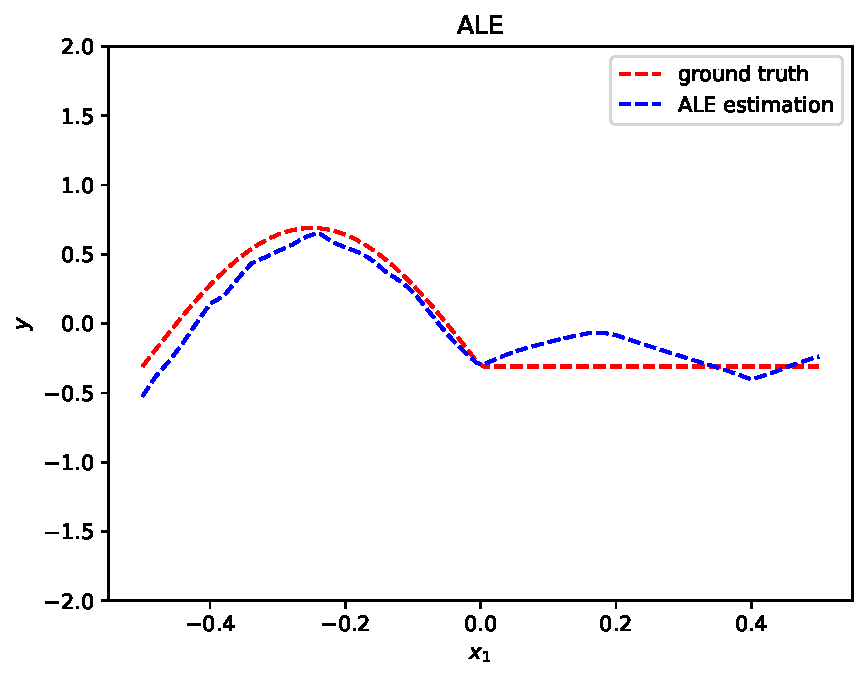
\includegraphics[width=1\textwidth]{concept_figure/exp_1_ale_50_bins_0}
%  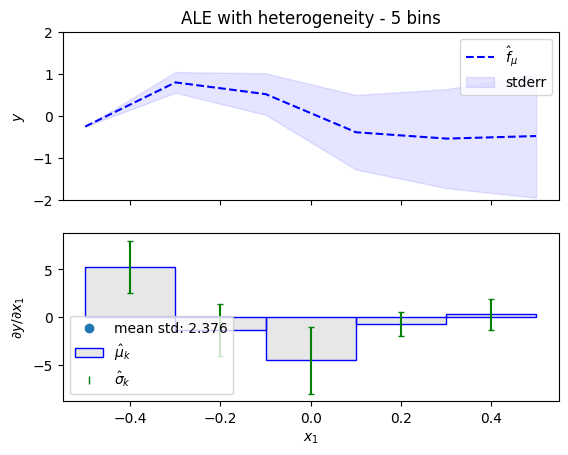
\includegraphics[width=1\textwidth]{concept_figure/exp_1_rhale_5_bins_0}
  \caption{ALE plot (50 fixed-size bins)}
  \label{fig:concept-figure-subfig-1-app}
\end{subfigure}%
\begin{subfigure}{.32\textwidth}
  \centering
  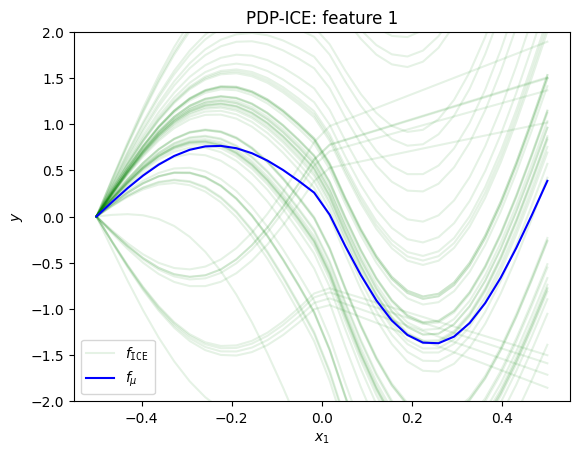
\includegraphics[width=1\textwidth]{concept_figure/exp_1_pdp_ice_0}
%  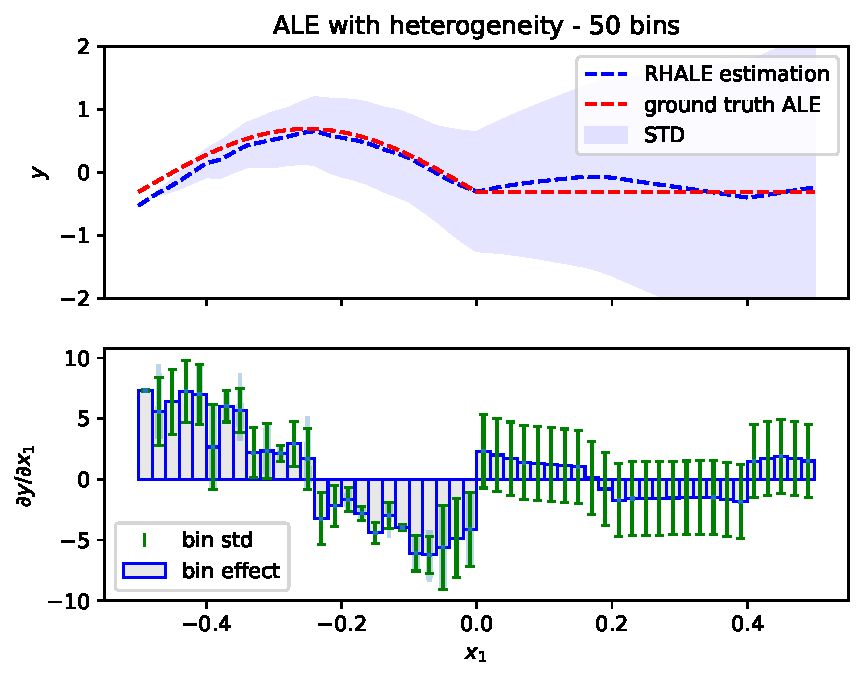
\includegraphics[width=1\textwidth]{concept_figure/exp_1_rhale_50_bins_0}\\
  \caption{PDP-ICE plot}
  \label{fig:concept-figure-subfig-2-app}
\end{subfigure}
\begin{subfigure}{.32\textwidth}
  \centering
  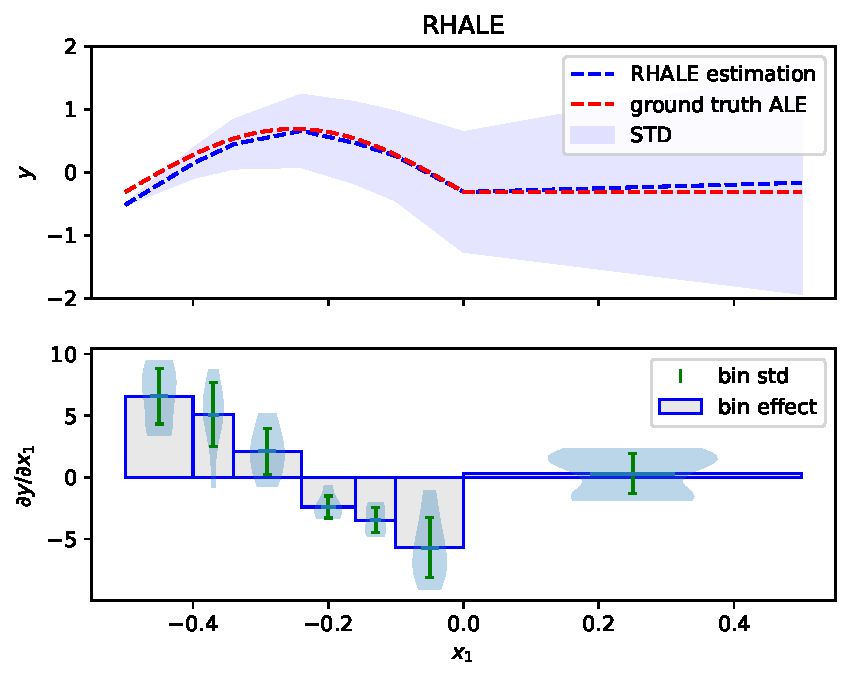
\includegraphics[width=1\textwidth]{concept_figure/exp_1_rhale_0}
  \caption{RHALE plot}
  \label{fig:concept-figure-subfig-3-app}
\end{subfigure}
\caption{Feature effect of $x_1$ on the example defined by Equation~\ref{eq:target_function-1}.
ALE does not quantify the heterogeneity and fixed-size splitting leads to a bad estimation.
PDP-ICE plots fail in both main effect and heterogeneity, failing to capture feature correlations.
RHALE, on the other hand, provides a robust estimation of the main effect and the heterogeneity.}
\label{fig:concept-figure-app}
\end{figure}

\subsection{Simulation Study}
\label{sec:simulation-study}

The data generating distribution is
\(p(\mathbf{x}) = p(x_3)p(x_2|x_1)p(x_1)\), where
\(x_1 \sim \mathcal{U}(0,1)\), \(x_2 = x_1 + \epsilon \), where $\epsilon \sim \mathcal{N}(0, 0.01)$ is a small additive, noise and
\(x_3 \sim \mathcal{N}(0, \sigma_3^2 = \frac{1}{4})\). The predictive function is:
%
\begin{equation}
  \label{eq:synth-ex-1-function-app}
  f(\mathbf{x}) = \underbrace{\alpha f_2(\xb)}_{g_3(\xb)} + \underbrace{f_1(\xb) \mathbbm{1}_{f_1(\xb) \leq \frac{1}{2}}}_{g_1(\xb)} + \underbrace{(1 - f_1(\xb)) \mathbbm{1}_{\frac{1}{2} < f_1(\xb) < 1}}_{g_2(\xb)}
\end{equation}
%
where \(f_1(\mathbf{x}) = a_1 x_1 + a_2 x_2\) is a linear combination of $x_1, x_2$, and
\(f_2(\mathbf{x}) = x_1 x_3\) interacts the non-correlated features $x_1, x_3$.
We evaluate the effect computed by RHALE and PDP-ICE in three cases; (a)
without interaction (\(\alpha=0\)) and equal weights (\(a_1=a_2\)),
(b) without interaction (\(\alpha=0\)) and different weights
(\( a_1 \neq a_2 \)) and (c) with interaction (\(\alpha > 0\)) and
equal weights (\(a_1=a_2\)).

%\paragraph{General description for all solutions}
\paragraph{Ground truth for case (a)}

In this case, the weights are $a_1 = a_2 = 1$ and there is no interaction term $\alpha=0$).
Therefore:

\begin{equation}
  \label{eq:case-a}
  f(\mathbf{x}) = f_1(\xb) \mathbbm{1}_{f_1(\xb) \leq \frac{1}{2}} + (1 - f_1(\xb)) \mathbbm{1}_{\frac{1}{2} < f_1(\xb) < 1}
\end{equation}
%
where $f_1(\xb) = x_1 + x_2$.
For the ground truth feature effect, we use the fact that $x_1 \approx x_2$,
therefore knowing only the value of $x_1$ we can automatically infer the value of $x_2$
and therefore the value of $f_1(\xb)$.
For example, when $0 \leq x_1 \leq \frac{1}{4}$ then $0 \leq f_1(\xb) \leq \frac{1}{2}$ and,
therefore, $f_1(x_1) = a_1 x_1$.
In a similar way, we compute the effect of $x_2$.
The effect of $x_3$ is zero.
%
\begin{align}
    \label{eq:case-a-feat-1}
    f^{\mathtt{GT}}(x_1) &= x_1 \mathbbm{1}_{0 \leq x_1 \leq \frac{1}{4}} + \left ( \frac{1}{4} - x_1 \right ) \mathbbm{1}_{\frac{1}{4} < x_1 < \frac{1}{2}} \\
    f^{\mathtt{GT}}(x_2) &= x_2 \mathbbm{1}_{0 \leq x_2 \leq \frac{1}{4}} + \left ( \frac{1}{4} - x_2 \right ) \mathbbm{1}_{\frac{1}{4} < x_2 < \frac{1}{2}} \\
    f^{\mathtt{GT}}(x_3) &= 0
\end{align}
%
The heterogeneity is zero for all features because the heterogeneity is induced by the variability
of the interaction terms and, since, $x_1 \approx x_2$, the terms
$\mathbbm{1}_{f_1(\xb) \leq \frac{1}{2}}$ and $\mathbbm{1}_{\frac{1}{2} < f_1(\xb) \leq 1}$, do not vary.
%
\begin{figure}
    \label{fig:case-a}
    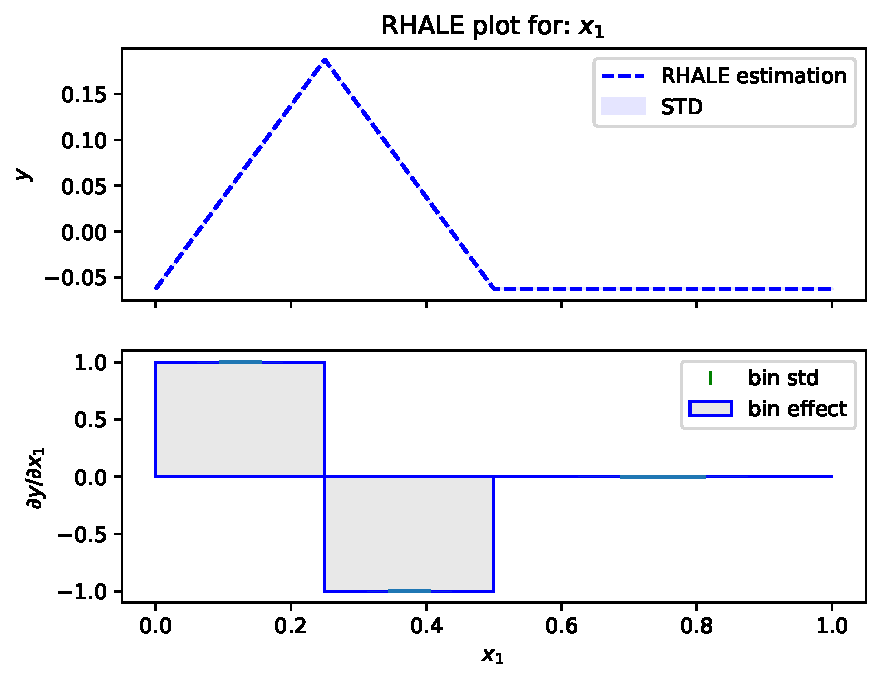
\includegraphics[width=0.3\linewidth]{example_1/dale_feat_0}
    \includegraphics[width=0.3\linewidth]{example_1/dale_feat_1}
    \includegraphics[width=0.3\linewidth]{example_1/dale_feat_2}\\
    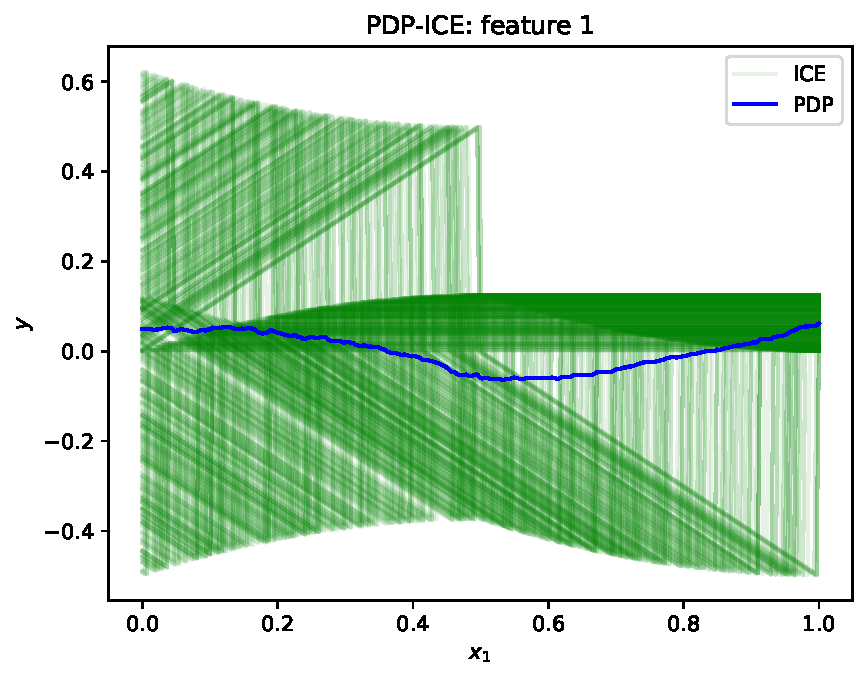
\includegraphics[width=0.3\linewidth]{example_1/pdp_ice_feat_0}
    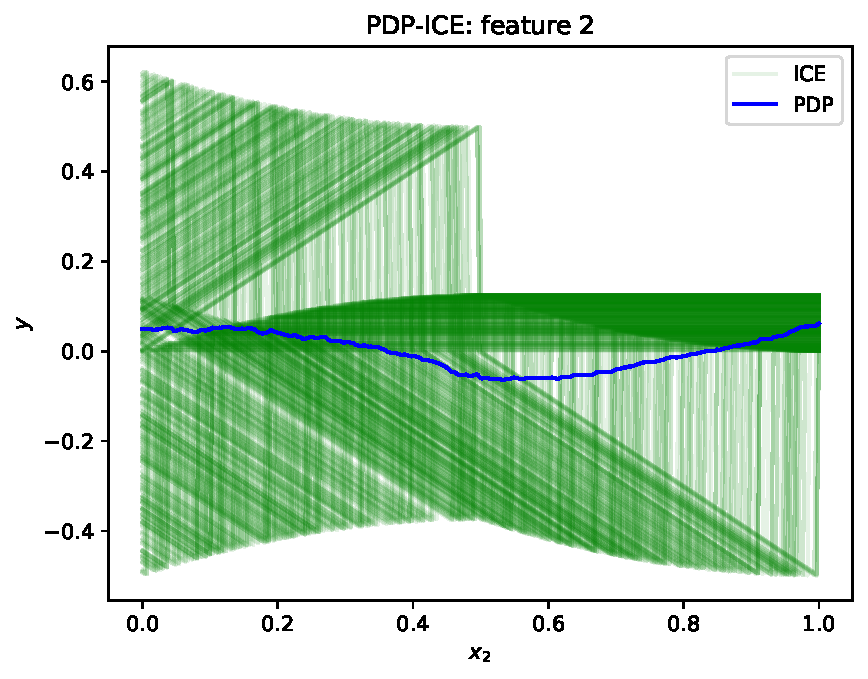
\includegraphics[width=0.3\linewidth]{example_1/pdp_ice_feat_1}
    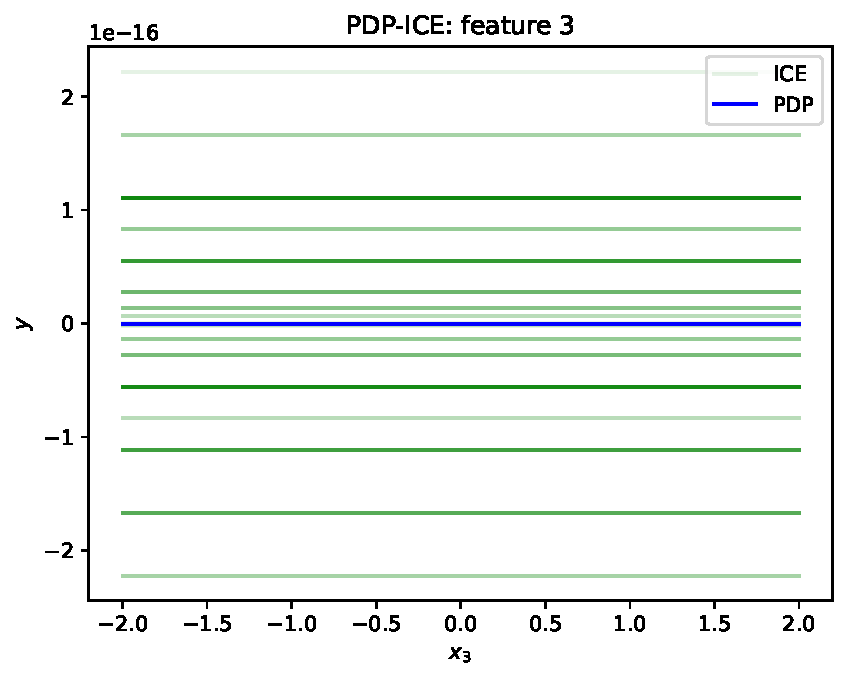
\includegraphics[width=0.3\linewidth]{example_1/pdp_ice_feat_2}
    \caption{Case (a)}
\end{figure}

\paragraph{Ground truth for case (b)}

In this case, the weights are $a_1 = 2$ and $a_2 = \frac{1}{2}$ and there is no interaction
term $\alpha=0$.
Therefore:

\begin{equation}
  \label{eq:case-b}
  f(\mathbf{x}) = f_1(\xb) \mathbbm{1}_{f_1(\xb) \leq \frac{1}{2}} + (1 - f_1(\xb)) \mathbbm{1}_{\frac{1}{2} < f_1(\xb) < 1}
\end{equation}
%
where $f_1(\xb) = 2 x_1 + \frac{1}{2} x_2$.
As in case (a), we use again the fact that $x_1 \approx x_2$,
to compute the ground truth feature effect:
%
\begin{align}
    \label{eq:case-b-app}
    f^{\mathtt{GT}}(x_1) &= 2 x_1 \mathbbm{1}_{0 \leq x_1 \leq \frac{1}{5}} + (\frac{2}{5} - 2 x_1) \mathbbm{1}_{\frac{1}{4} < x_1 < \frac{2}{5}} \\
    f^{\mathtt{GT}}(x_2) &= 2 x_2 \mathbbm{1}_{0 \leq x_2 \leq \frac{1}{5}} + (\frac{2}{5} - 2 x_2) \mathbbm{1}_{\frac{1}{4} < x_2 < \frac{2}{5}} \\
    f^{\mathtt{GT}}(x_3) &= 0
\end{align}
%
The heterogeneity is zero for all features because the heterogeneity is induced by the variability
of the interaction terms and, since, $x_1 \approx x_2$, the terms
$\mathbbm{1}_{f_1(\xb) \leq \frac{1}{2}}$ and $\mathbbm{1}_{\frac{1}{2} < f_1(\xb) \leq 1}$, do not vary.
%
\begin{figure}
    \label{fig:case-b}
    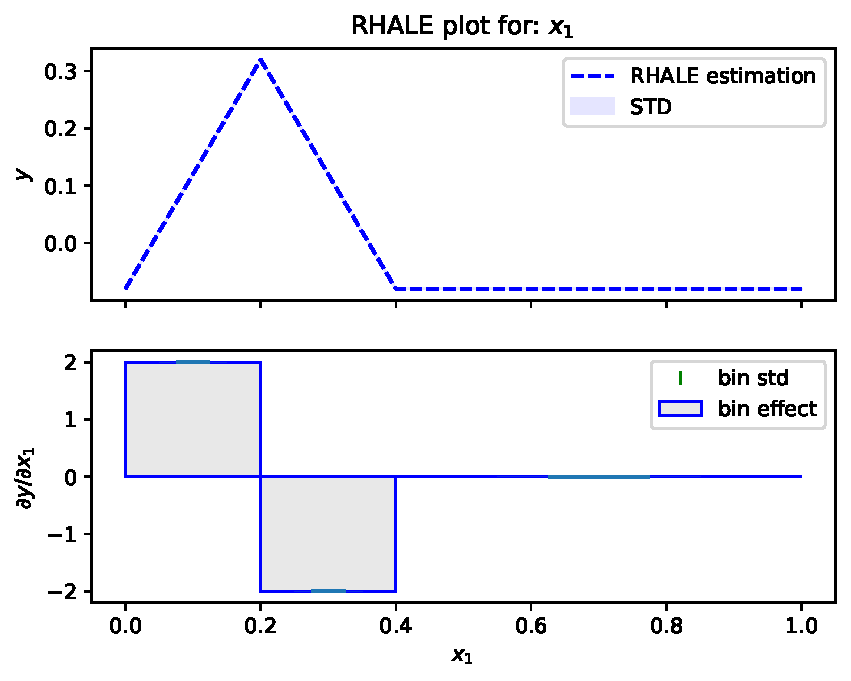
\includegraphics[width=0.3\linewidth]{example_2/dale_feat_0}
    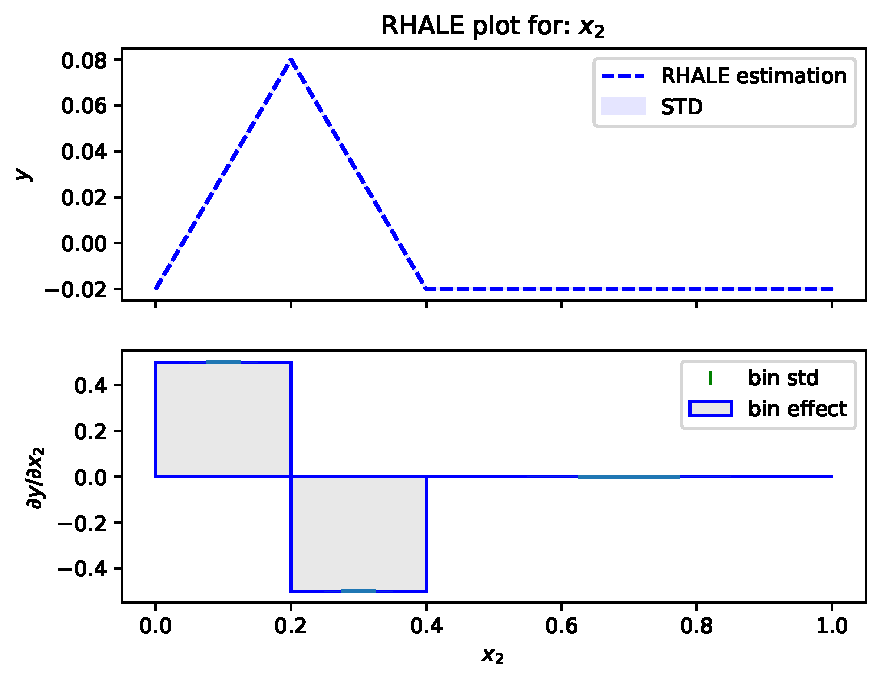
\includegraphics[width=0.3\linewidth]{example_2/dale_feat_1}
    \includegraphics[width=0.3\linewidth]{example_2/dale_feat_2}\\
    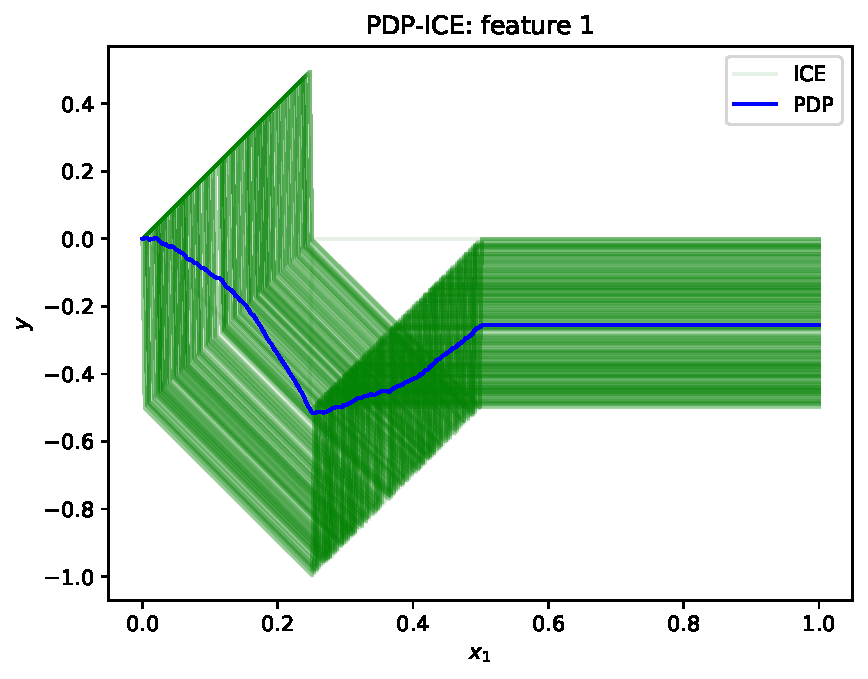
\includegraphics[width=0.3\linewidth]{example_2/pdp_ice_feat_0}
    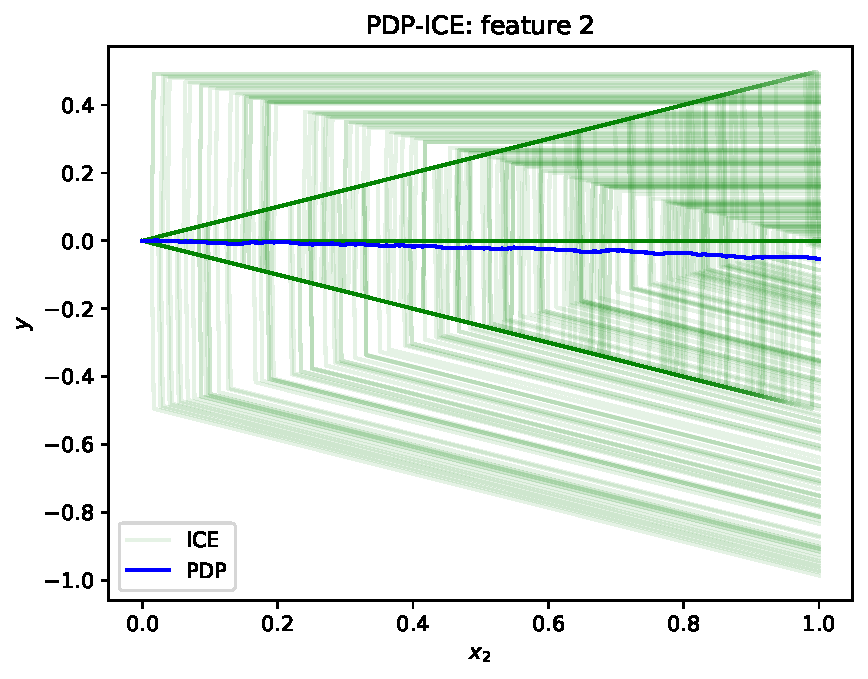
\includegraphics[width=0.3\linewidth]{example_2/pdp_ice_feat_1}
    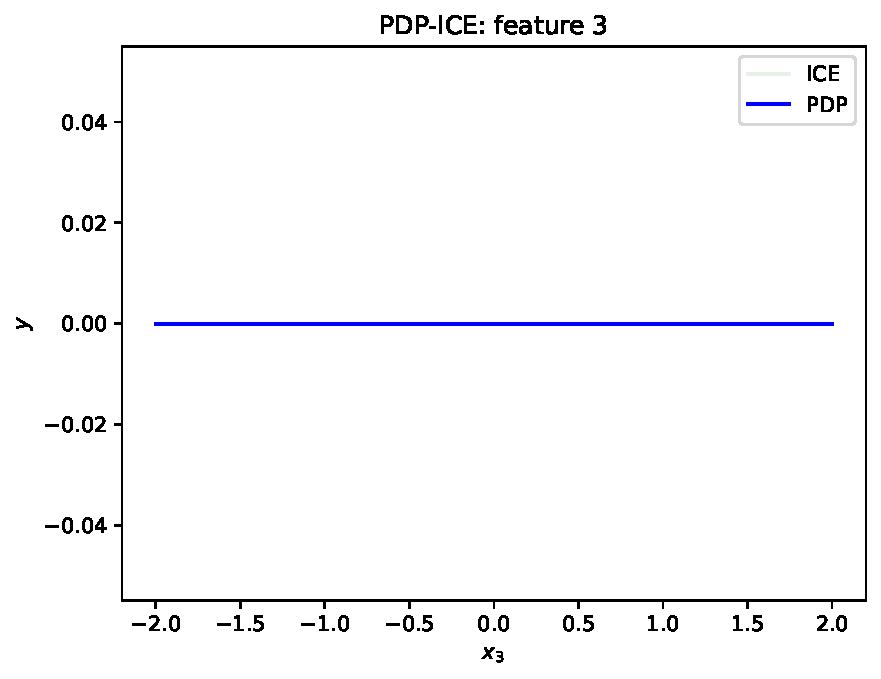
\includegraphics[width=0.3\linewidth]{example_2/pdp_ice_feat_2}
    \caption{Case (b)}
\end{figure}

\paragraph{Ground truth for case (c)}

In this case, the weights are equal $a_1 = a_2 = 1$ and the is interaction
term is enabled $(\alpha=1)$.
Therefore:

\begin{equation}
  \label{eq:case-c}
  f(\mathbf{x}) = f_2(\xb) + f_1(\xb) \mathbbm{1}_{f_1(\xb) \leq \frac{1}{2}} + (1 - f_1(\xb)) \mathbbm{1}_{\frac{1}{2} < f_1(\xb) < 1}
\end{equation}
%
where $f_2(\xb) = x_1 x_3$ and $f_1(\xb) = x_1 + x_2$.
The feature effect of terms
$f_1(\xb) \mathbbm{1}_{f_1(\xb) \leq \frac{1}{2}} + (1 - f_1(\xb)) \mathbbm{1}_{\frac{1}{2} < f_1(\xb) < 1}$
are exactly the same with case (a).
The term $f_2(\xb) = x_1 x_2$.
For feature $x_1$ the effect is $\mathbb{E}_{x_3|x_1} [x_1 x_3] = x_1 \mathbb{E}_{x_3} [x_3] = 0$ and
for feature $x_2$ the effect is $\mathbb{E}_{x_1|x_3} [x_1 x_3] = x_3 \mathbb{E}_{x_1} [x_1] = 0.5 x_3$.
Therefore, the ground truth feature effect is:
%
\begin{align}
    \label{eq:case-c-app}
    f^{\mathtt{GT}}(x_1) &= x_1 \mathbbm{1}_{0 \leq x_1 \leq \frac{1}{4}} + \left ( \frac{1}{4} - x_1 \right ) \mathbbm{1}_{\frac{1}{4} < x_1 < \frac{1}{2}} \\
    f^{\mathtt{GT}}(x_2) &= x_2 \mathbbm{1}_{0 \leq x_2 \leq \frac{1}{4}} + \left ( \frac{1}{4} - x_2 \right ) \mathbbm{1}_{\frac{1}{4} < x_2 < \frac{1}{2}} \\
    f^{\mathtt{GT}}(x_3) &= \frac{1}{2} x_3
\end{align}
%
For the same reason with cases (a) and (b), the terms
$\mathbbm{1}_{f_1(\xb) \leq \frac{1}{2}}$ and $\mathbbm{1}_{\frac{1}{2} < f_1(\xb) \leq 1}$,
do not introduce heterogeneity.
Since $x_1, x_2$ are independent the effect of $x_1 x_3$ varies.
For feature $x_1$, it varies following the standard deviation of $x_3$, i.e. $\sigma_3=\frac{1}{2}$ and
for feature $x_3$, it varies following the standard deviation of $x_1$, i.e. $\sigma_1=\frac{1}{4}$.
%
\begin{figure}
    \label{fig:case-c}
    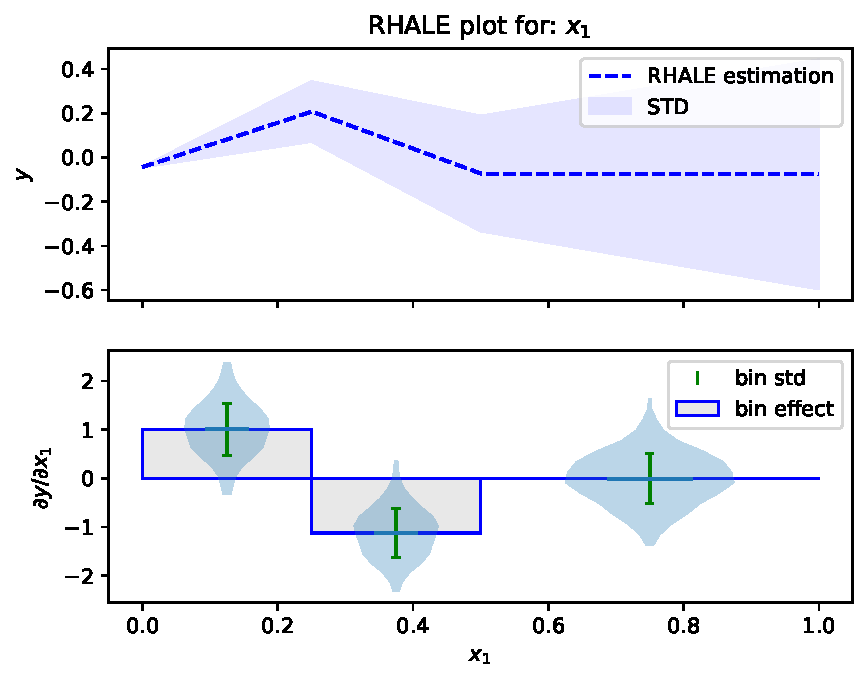
\includegraphics[width=0.3\linewidth]{example_3/dale_feat_0}
    \includegraphics[width=0.3\linewidth]{example_3/dale_feat_1}
    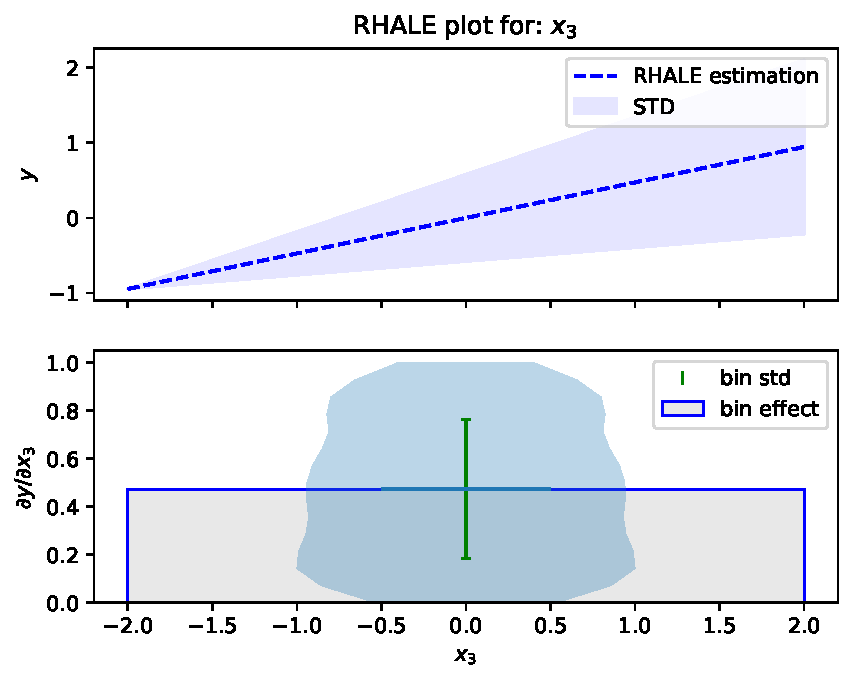
\includegraphics[width=0.3\linewidth]{example_3/dale_feat_2}\\
    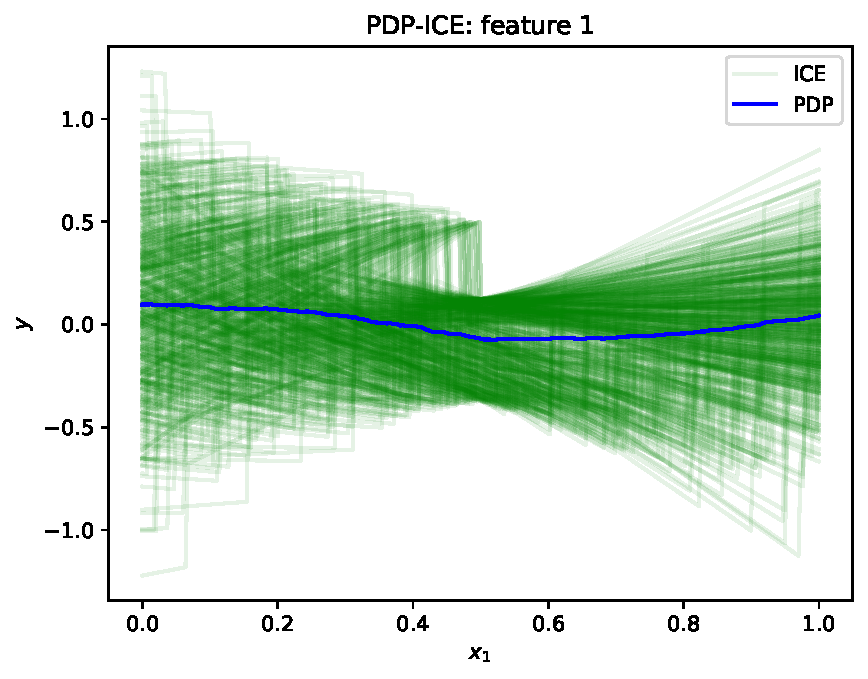
\includegraphics[width=0.3\linewidth]{example_3/pdp_ice_feat_0}
    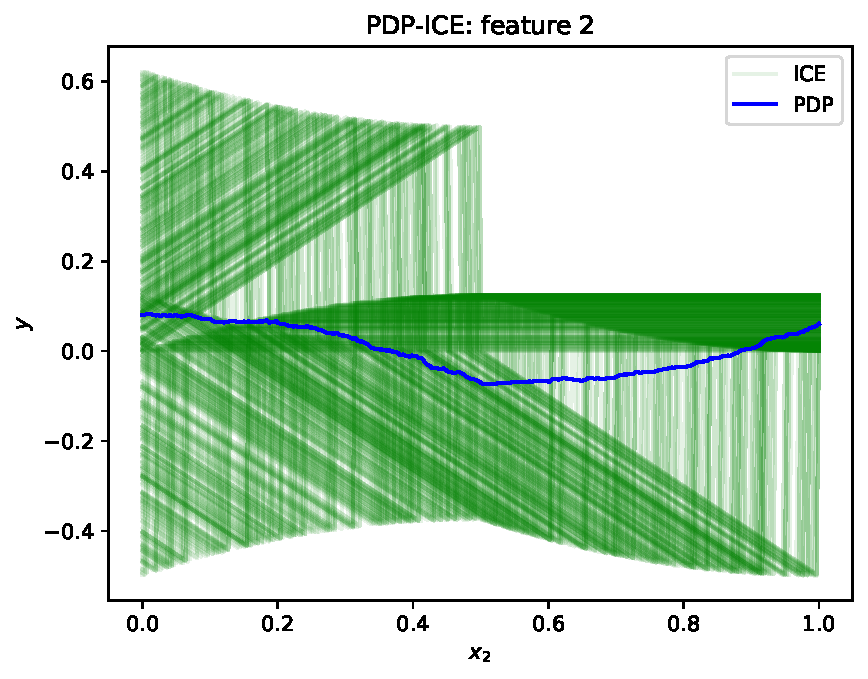
\includegraphics[width=0.3\linewidth]{example_3/pdp_ice_feat_1}
    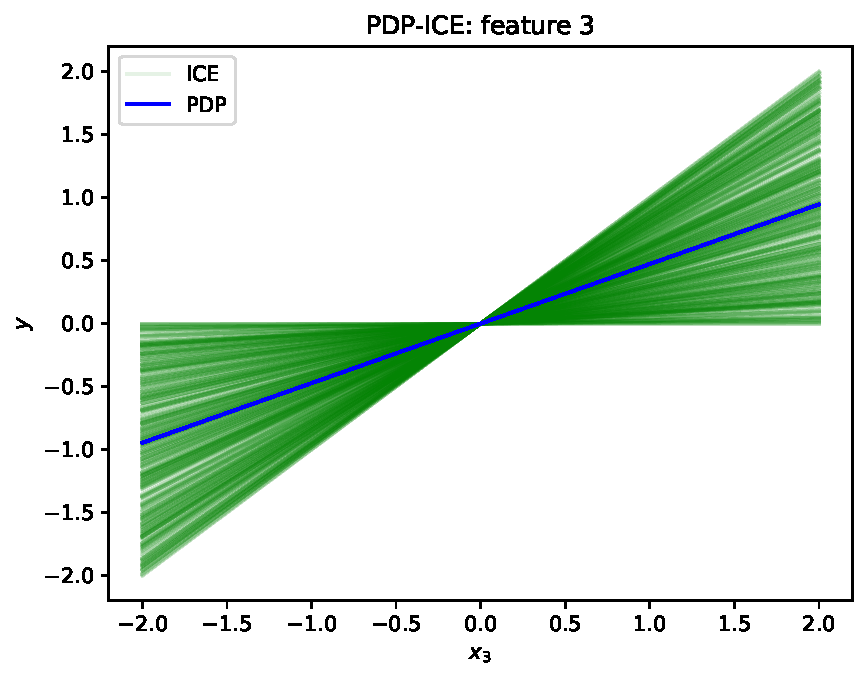
\includegraphics[width=0.3\linewidth]{example_3/pdp_ice_feat_2}
    \caption{Case (b)}
\end{figure}

\paragraph{Conclusion.}

The example confirms our previous knowledge that PDP-ICE provide erroneous
effects in cases with correlated features.
The feature effect computed by PDP and the heterogeneity illustrated by
ICE are correct only for feature $x_3$,
because it is independent from the other features.
For features the correlated features $x_1, x_2$,
both PDP and ICE provide misleading explanations.
In contrast, RHALE handles well all cases, providing accurate estimations for the feature effects
and the heterogeneity.

\subsection{Real World Experiment}
\label{sec:real-world-experiment}

In this section, we provide further details on the real-world
example.
The real-world example uses the California Housing Dataset,
which contains 8 numerical features. We exclude instances with missing
or outlier values. If we denote as \(\mu_s\) (\(\sigma_s\)) the
average value (standard deviation) of the \(s\)-th feature, we
consider outliers the instances of the training set with any feature
value over three standard deviations from the mean, i.e.
\(|x_s^i - \mu_s| > \sigma_s\). This preprocessing step discards
\(884\) instances, and \(N=19549\) remain. We provide their
description with some basic descriptive statistics in
Table~\ref{tab:features-description} and their histogram in
Figure~\ref{fig:feature-histograms}.

In Figure 7 of the main paper, we provided the RHALE vs PDP-ICE plots
for features \(x_2\) (latitude), \(x_6\) (total number of people) and
\(x_8\) (median house value). In figure 8, we compared RHALE with
fixed-size approximation, for the same features. In
Figure~\ref{fig:ex-real-1-app}, we provide the same information for the
rest of the features; \(x_1\) (longitude), \(x_3\) (median age of
houses), \(x_4\) (total number of rooms), \(x_5\) (total number of
bedrooms) and \(x_7\) (total number of households). The observation of
these features leads us to similar conclusion. First, RHALE and
PDP-ICE plots compute similar effects and level of heterogeneity and
RHALE's approximation is (almost) as good as the best fixed-size
approximation. More specifically, we observe that RHALE's variable size
bin splitting correctly creates wide bins for features
\(x_3, x_4, x_5, x_7\), where the feature effect plot is (piecewise)
linear, while using narrow bins for feature \(x_2\) where the feature
effect is not linear.

\begin{table}
  \caption{Description of the features apparent in the California-Housing Dataset}
  \label{tab:features-description}
  \centering
  \begin{tabular}{ c|c|c|c|c|c| }
    \hline
    & Description & \(min\) & \(\max\) & \(\mu\) & \(\sigma\) \\
    \hline
    \(x_1\) & longitude & \(-124.35\) & \(-114.31\) & \(-119.58\) & \(2\) \\
    \(x_2\) & latitude  & \(32.54\) & \(41.95\) & \(35.65\) & \(2.14\) \\
    \(x_3\) & median age of houses & \(1\) & \(52\) & \(29.01\) & \(12.42\) \\
    \(x_4\) & total number of rooms & \(2\) & \(9179\) & \(2390.79\) & \(1433.83\) \\
    \(x_5\) & total number of bedrooms & \(2\) & \(1797\) & \(493.86\) & \(291\) \\
    \(x_6\) & total number of people & \(3\) & \(4818\) & \(1310.91\) & \(771.78\) \\
    \(x_7\) & total number of households & \(2\) & \(1644\) & \(460.3\) & \(267.34\) \\
    \(x_8\) & median income of households & \(0.5\) & \(9.56\) & \(3.72\) & \(1.60\) \\
    \hline
    \(y\) & median house value & \(14.999\) & \(500000\) & \(206864.41\) & \(115435.67\) \\
    \hline
  \end{tabular}
\end{table}


\begin{figure}[h]
  \centering
  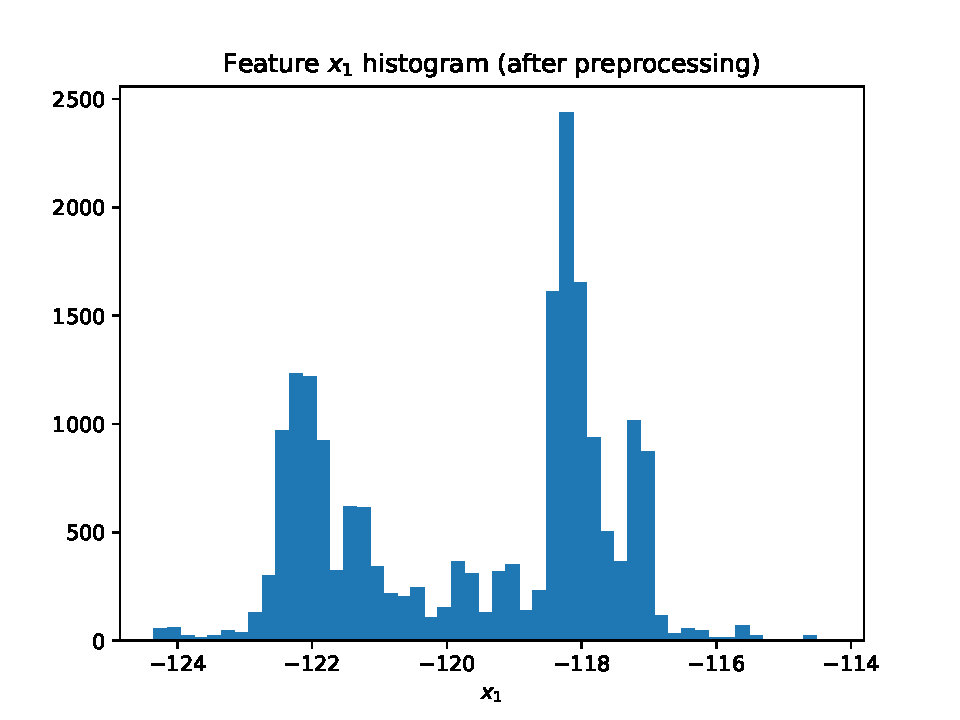
\includegraphics[width=.43\textwidth]{real_dataset_3/hist_feat_1_after}
  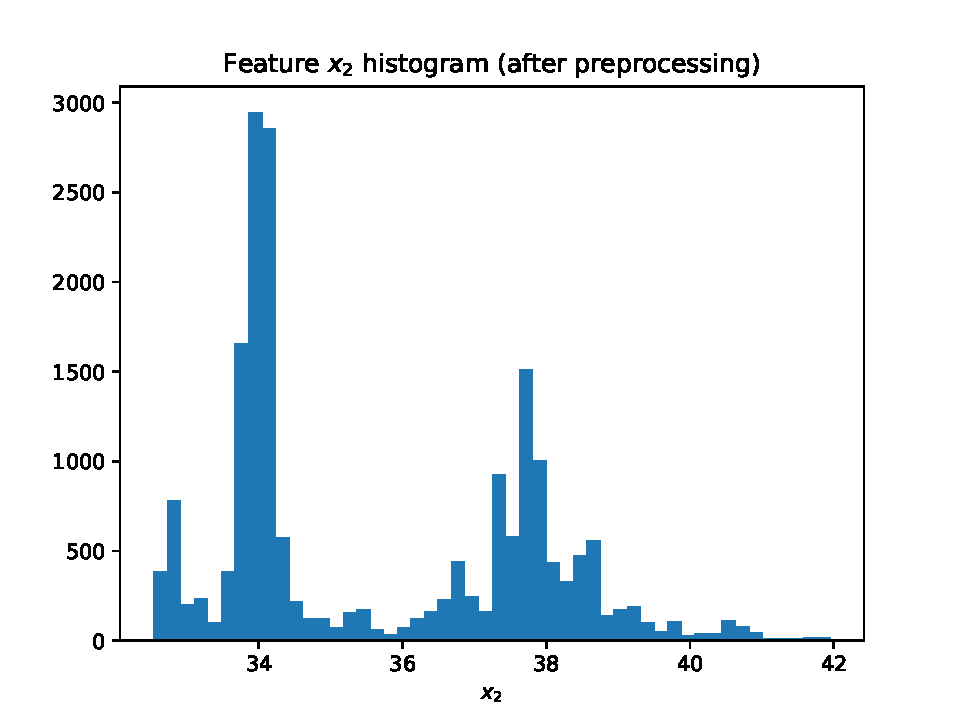
\includegraphics[width=.43\textwidth]{real_dataset_3/hist_feat_2_after}\\
  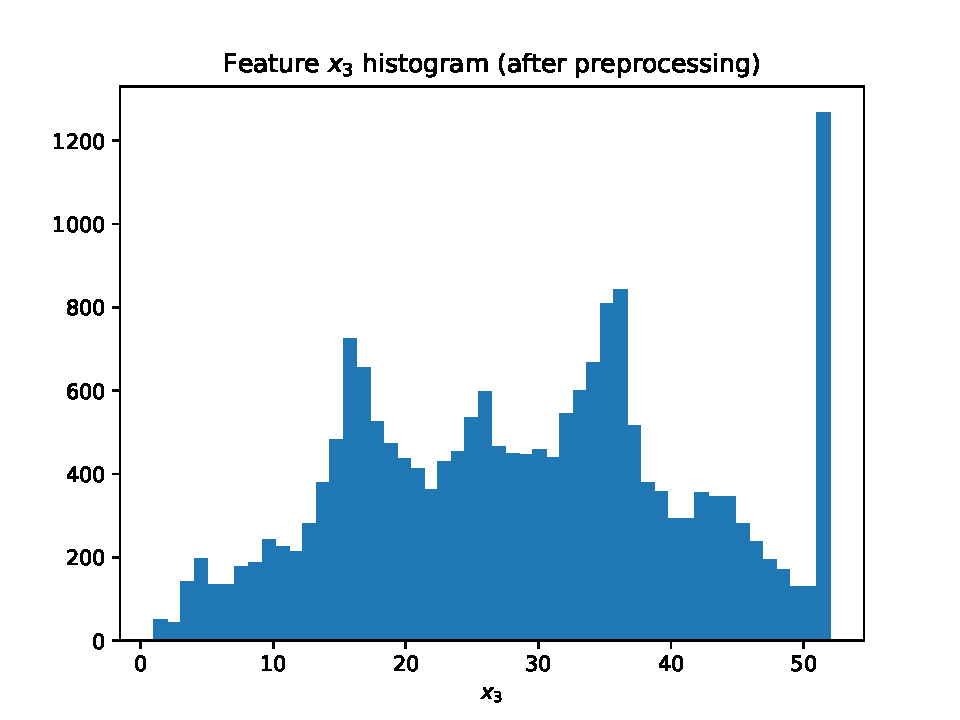
\includegraphics[width=.43\textwidth]{real_dataset_3/hist_feat_3_after}
  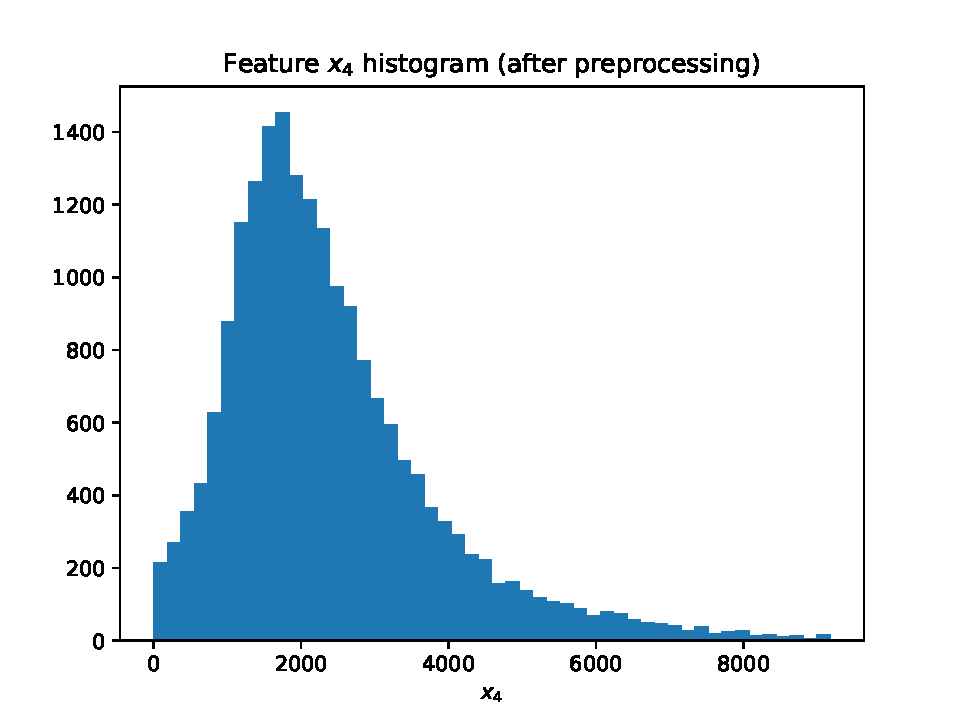
\includegraphics[width=.43\textwidth]{real_dataset_3/hist_feat_4_after}\\
  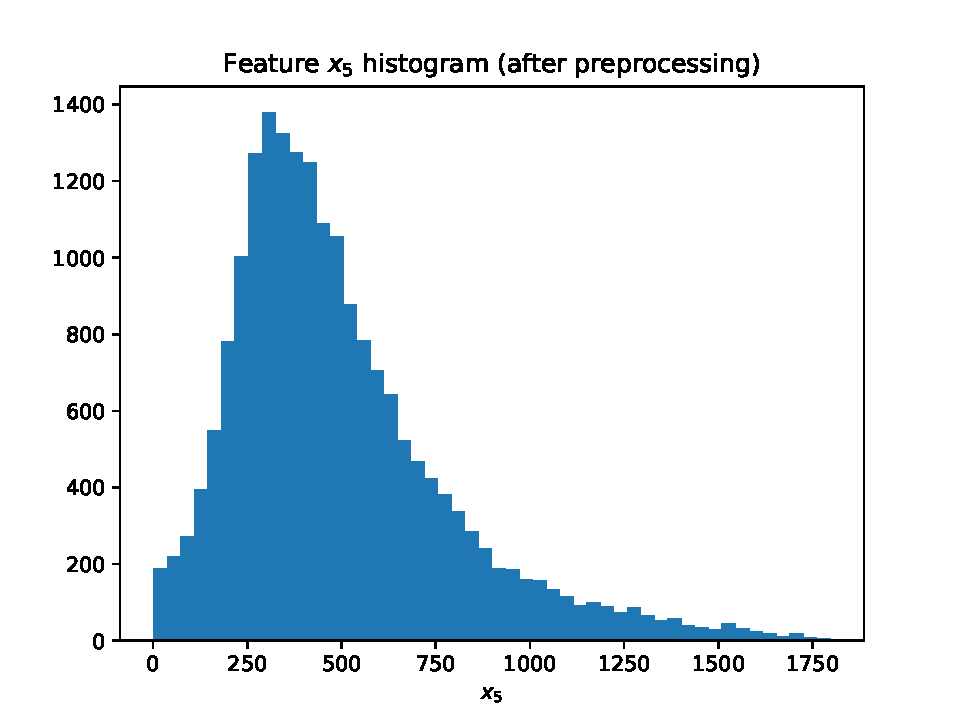
\includegraphics[width=.43\textwidth]{real_dataset_3/hist_feat_5_after}
  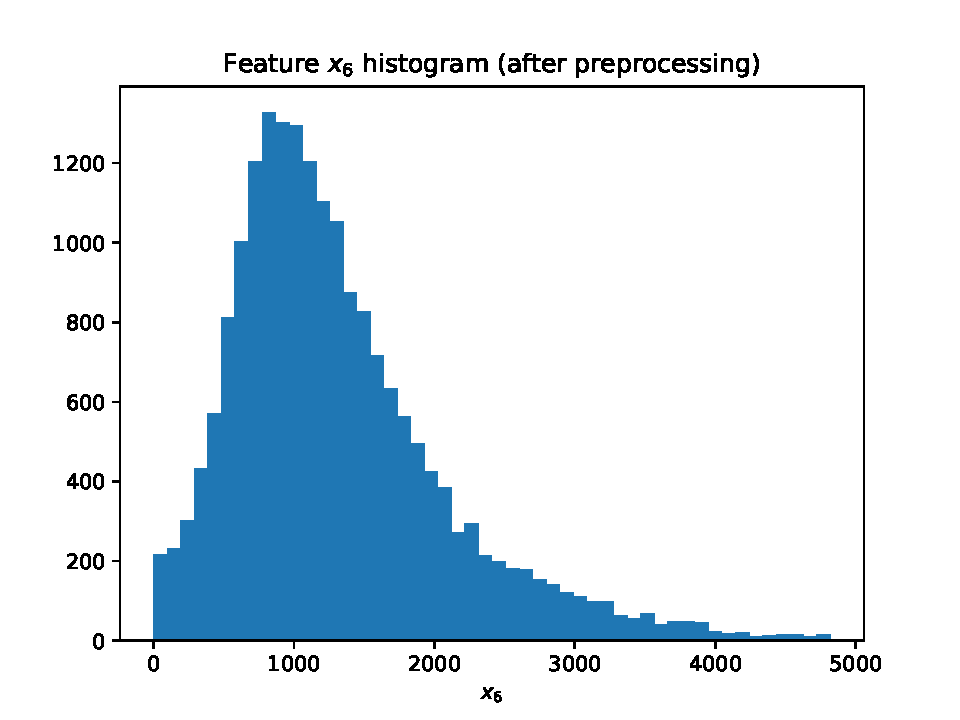
\includegraphics[width=.43\textwidth]{real_dataset_3/hist_feat_6_after}\\
  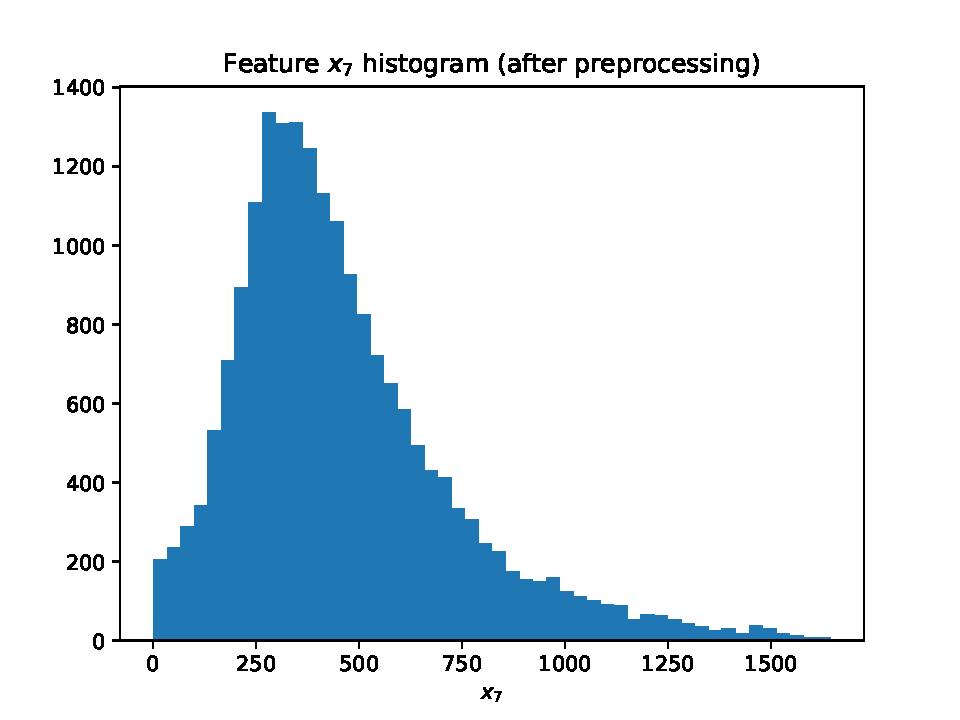
\includegraphics[width=.43\textwidth]{real_dataset_3/hist_feat_7_after}
  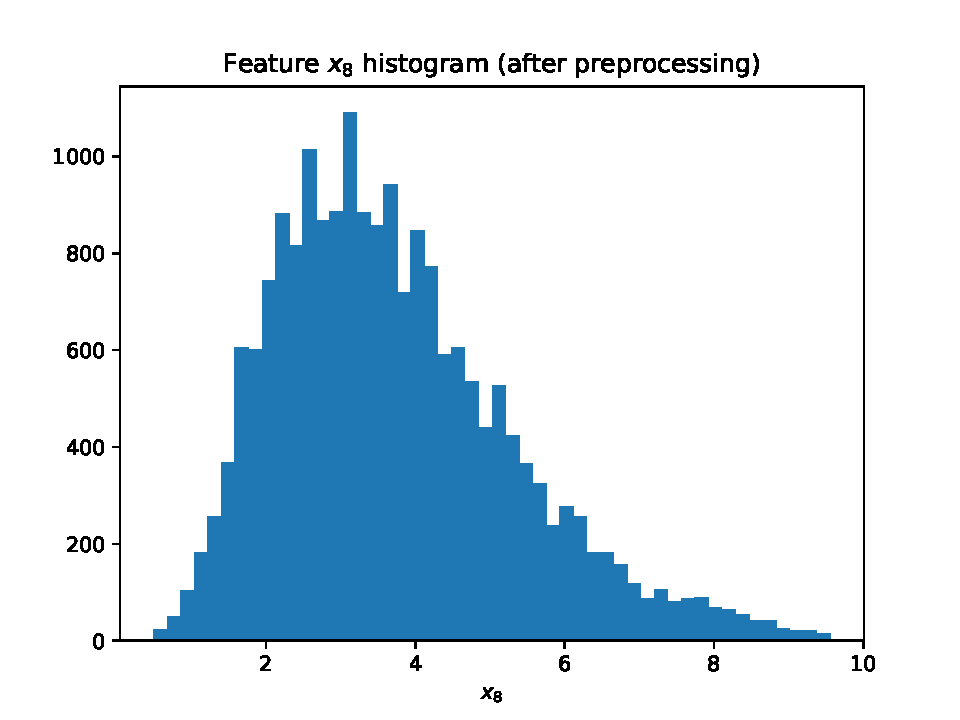
\includegraphics[width=.43\textwidth]{real_dataset_3/hist_feat_8_after}\\
  \caption{The Histogram of each feature in the California Housing Dataset.}
  \label{fig:feature-histograms}
\end{figure}



\begin{figure}[h]
  \centering
  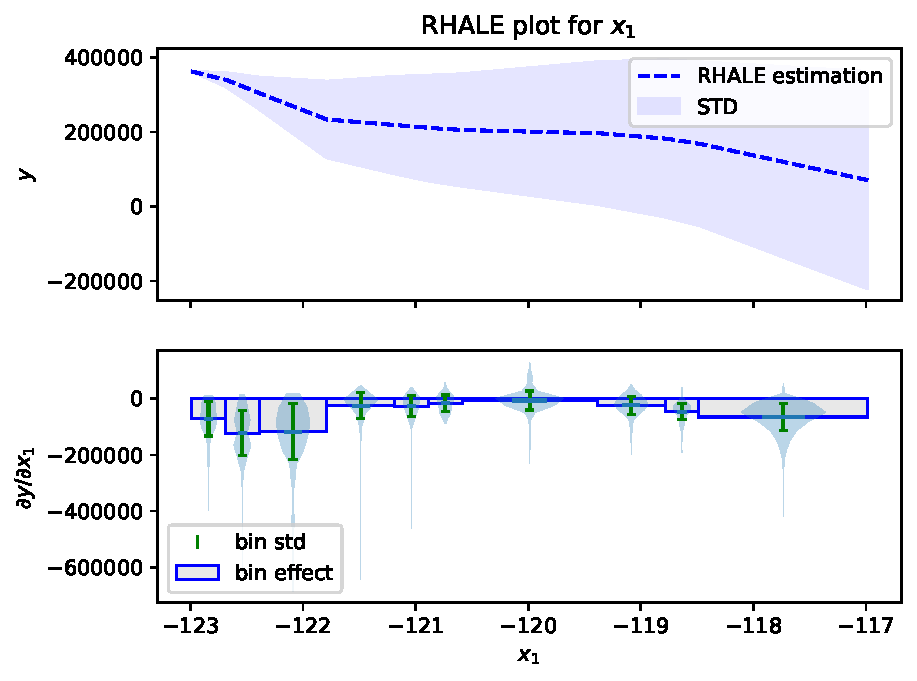
\includegraphics[width=.24\textwidth]{real_dataset_3/feature_0_ale_auto}
  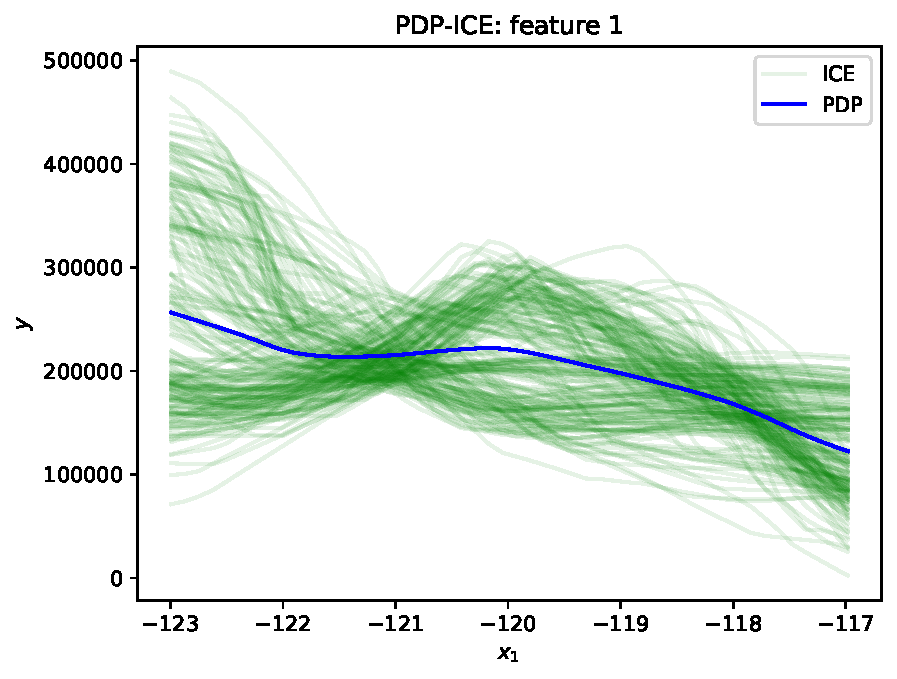
\includegraphics[width=.24\textwidth]{real_dataset_3/feature_0_pdp_ice}
  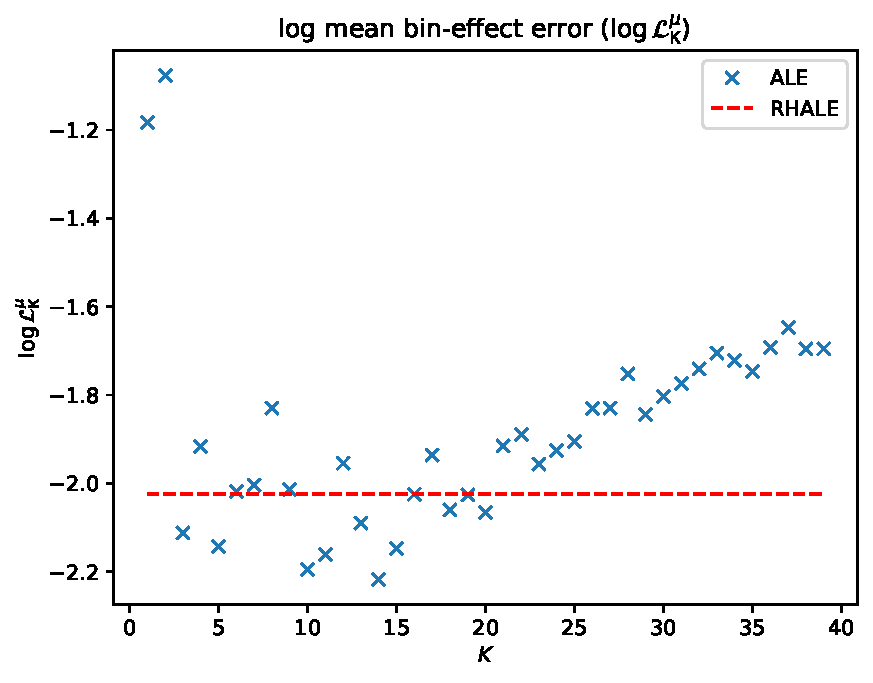
\includegraphics[width=.24\textwidth]{real_dataset_3/compare_mu_err_feature_0}
  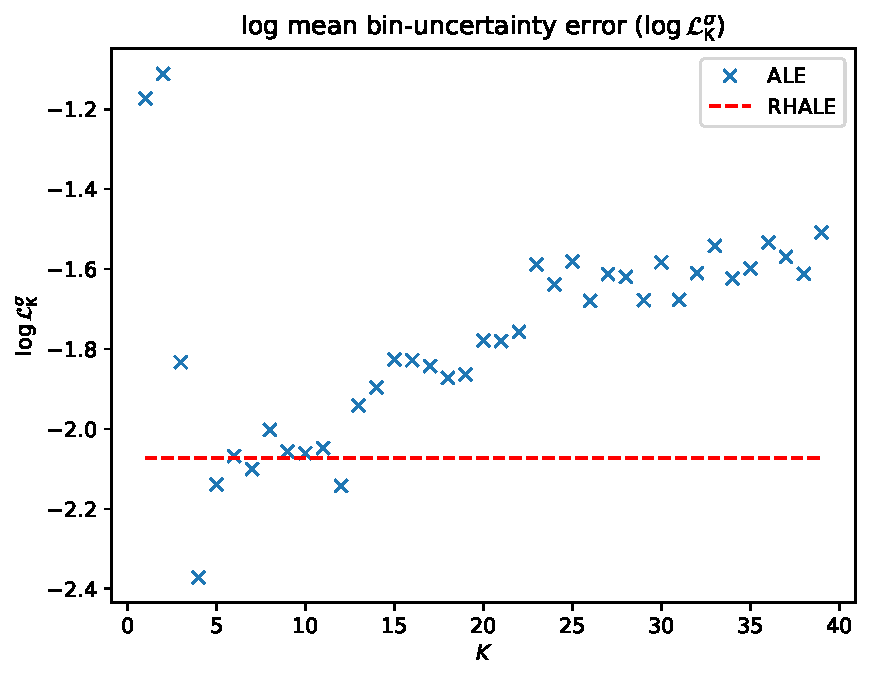
\includegraphics[width=.24\textwidth]{real_dataset_3/compare_var_err_feature_0}\\
  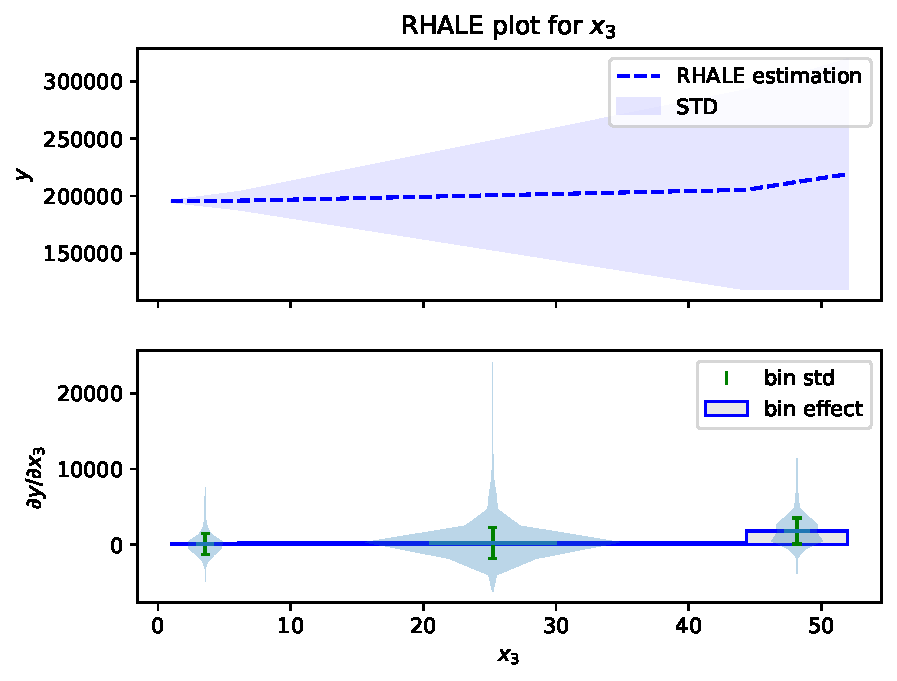
\includegraphics[width=.24\textwidth]{real_dataset_3/feature_2_ale_auto}
  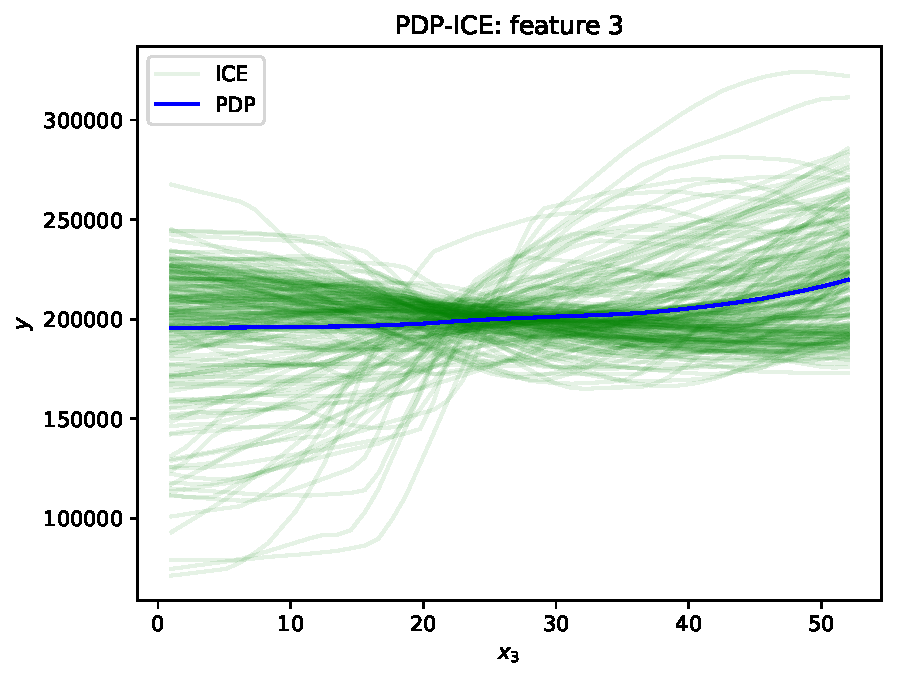
\includegraphics[width=.24\textwidth]{real_dataset_3/feature_2_pdp_ice}
  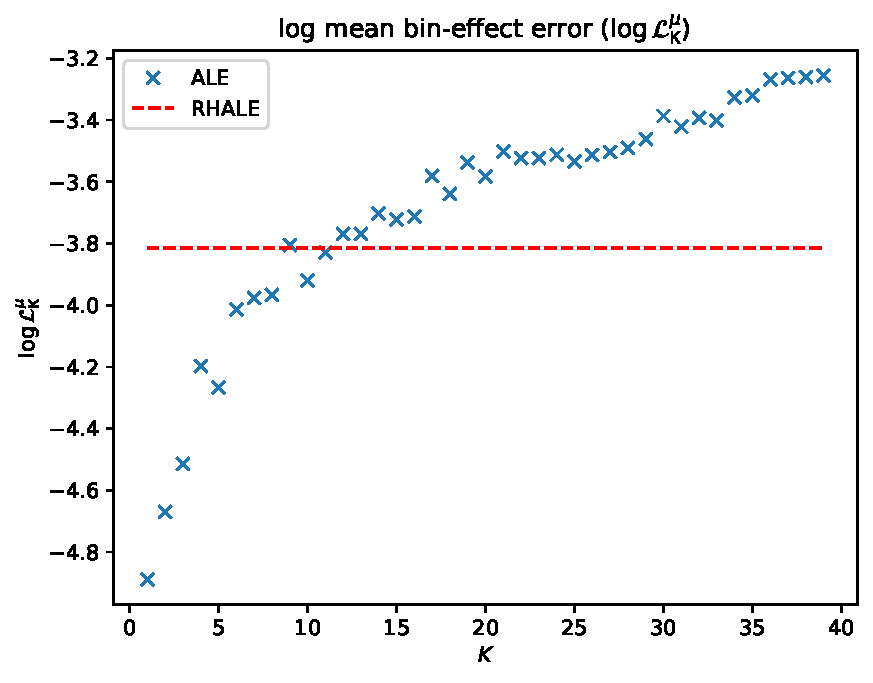
\includegraphics[width=.24\textwidth]{real_dataset_3/compare_mu_err_feature_2}
  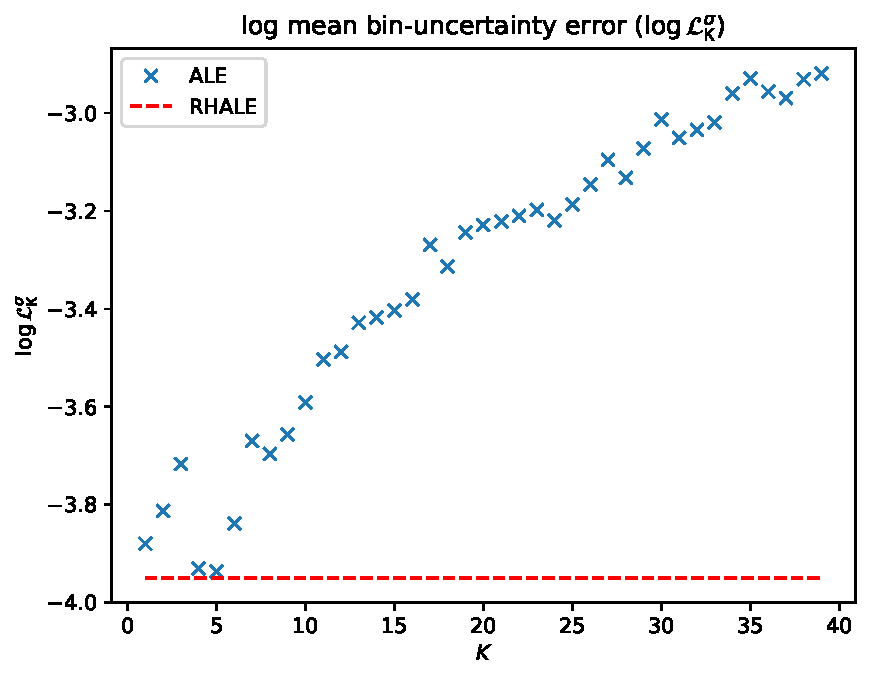
\includegraphics[width=.24\textwidth]{real_dataset_3/compare_var_err_feature_2}\\
  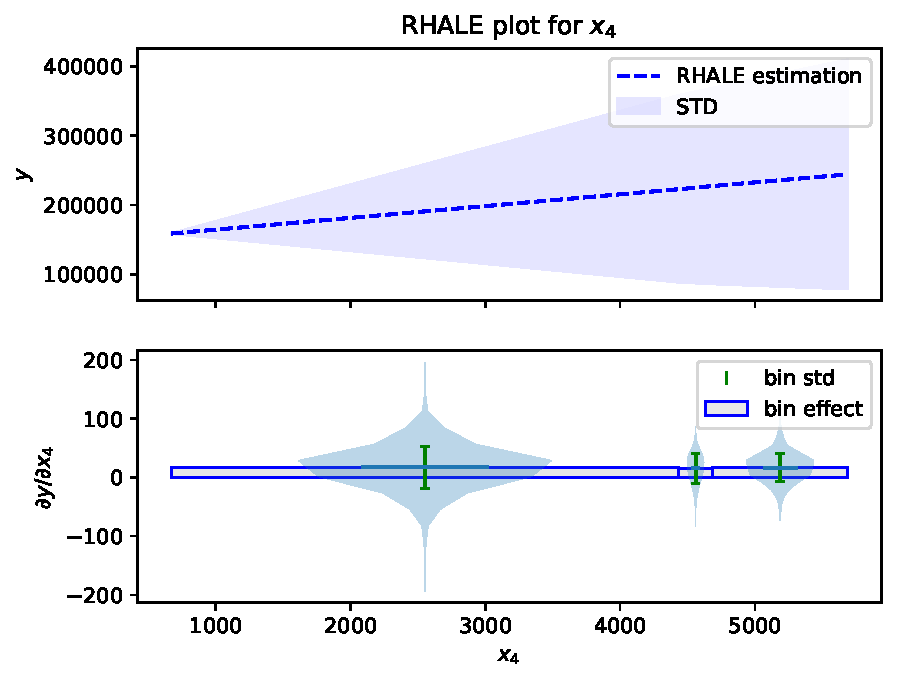
\includegraphics[width=.24\textwidth]{real_dataset_3/feature_3_ale_auto}
  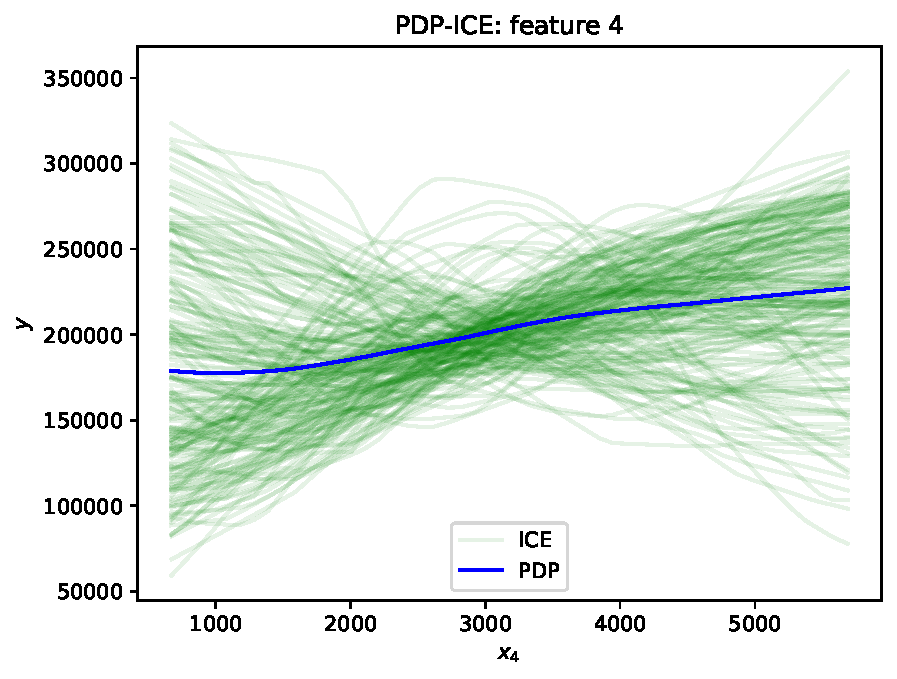
\includegraphics[width=.24\textwidth]{real_dataset_3/feature_3_pdp_ice}
  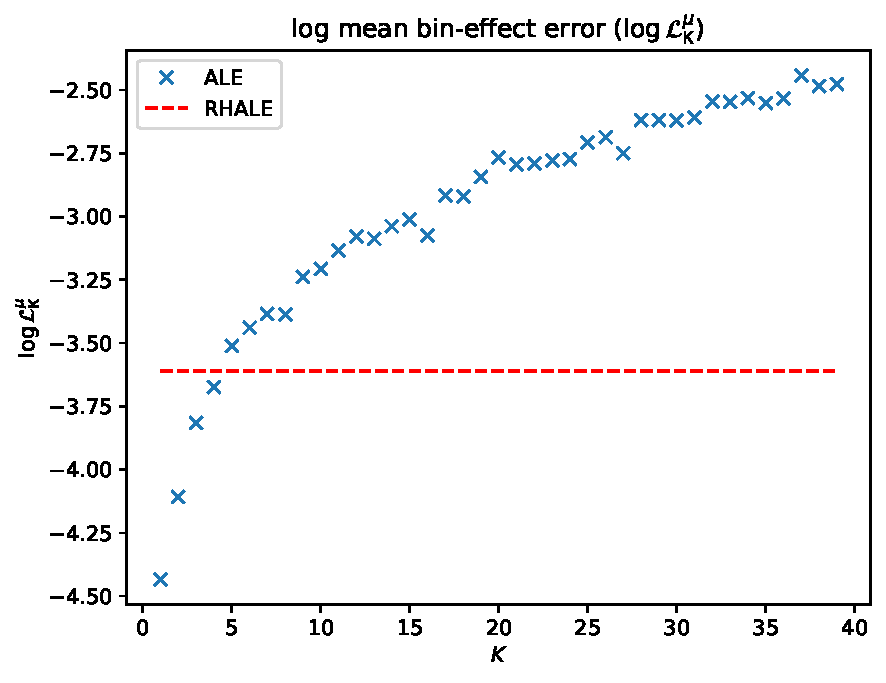
\includegraphics[width=.24\textwidth]{real_dataset_3/compare_mu_err_feature_3}
  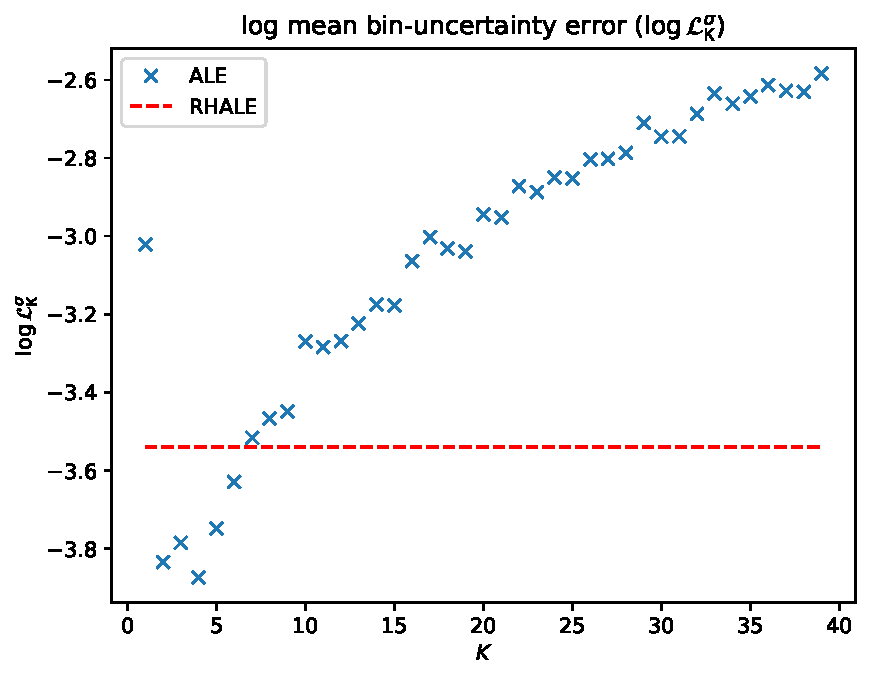
\includegraphics[width=.24\textwidth]{real_dataset_3/compare_var_err_feature_3}\\
  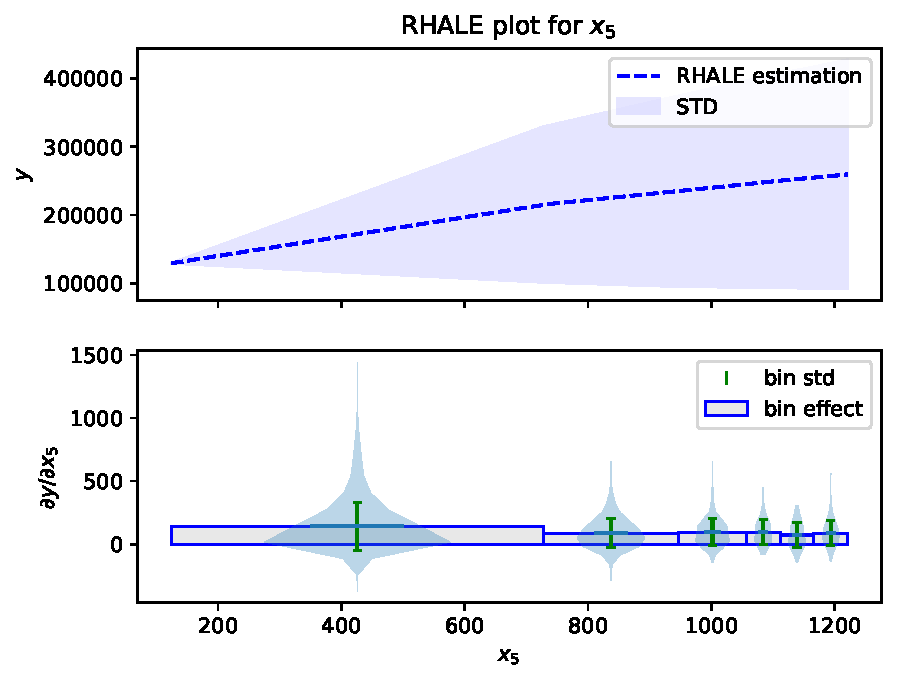
\includegraphics[width=.24\textwidth]{real_dataset_3/feature_4_ale_auto}
  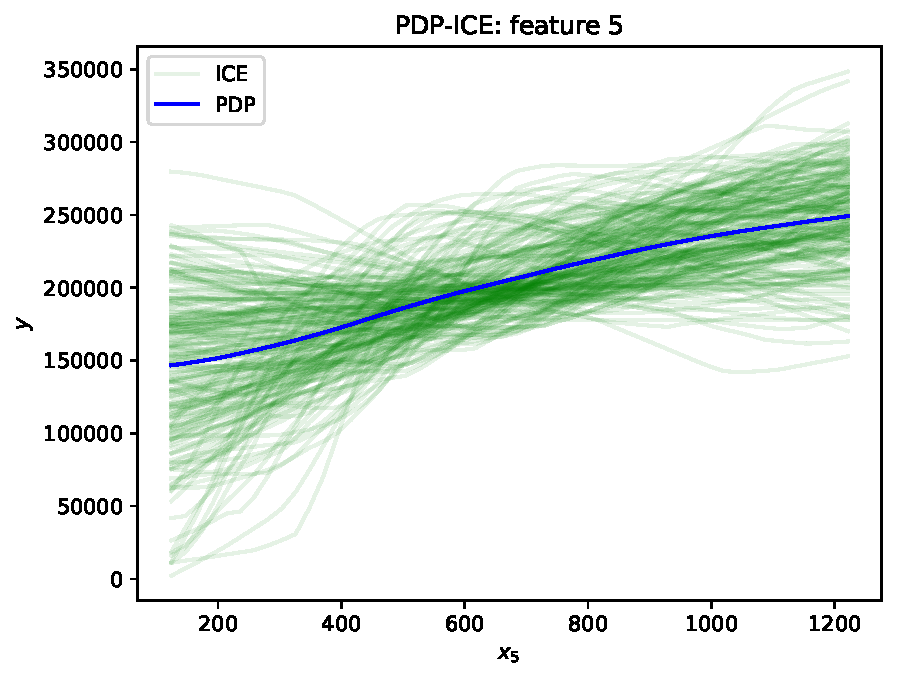
\includegraphics[width=.24\textwidth]{real_dataset_3/feature_4_pdp_ice}
  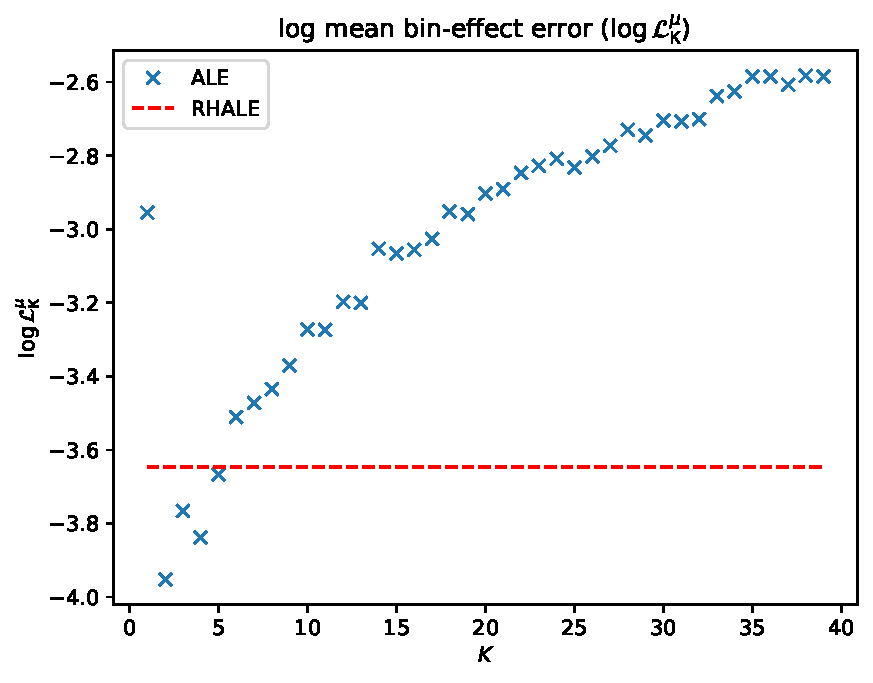
\includegraphics[width=.24\textwidth]{real_dataset_3/compare_mu_err_feature_4}
  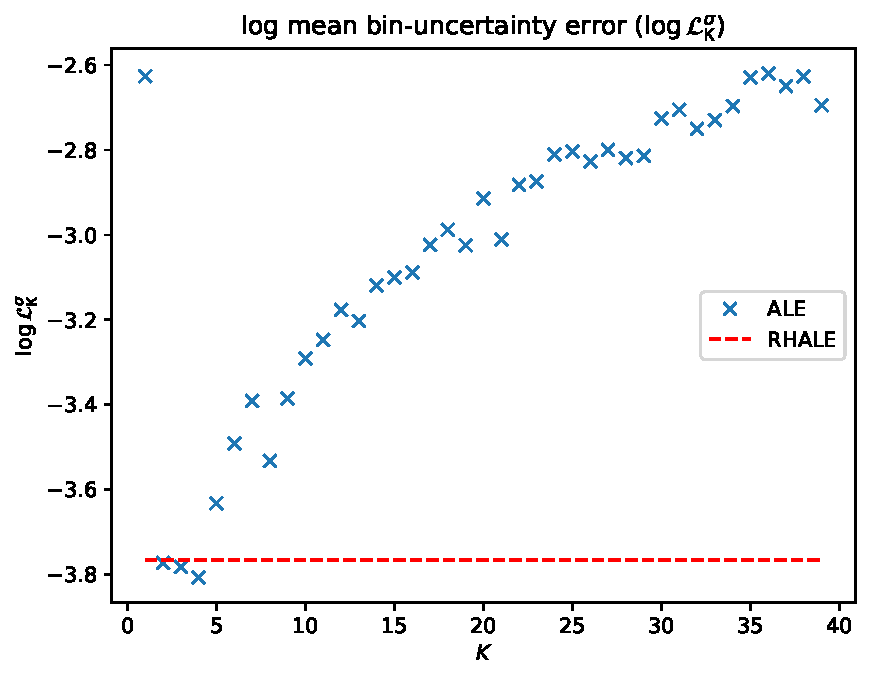
\includegraphics[width=.24\textwidth]{real_dataset_3/compare_var_err_feature_4}\\
  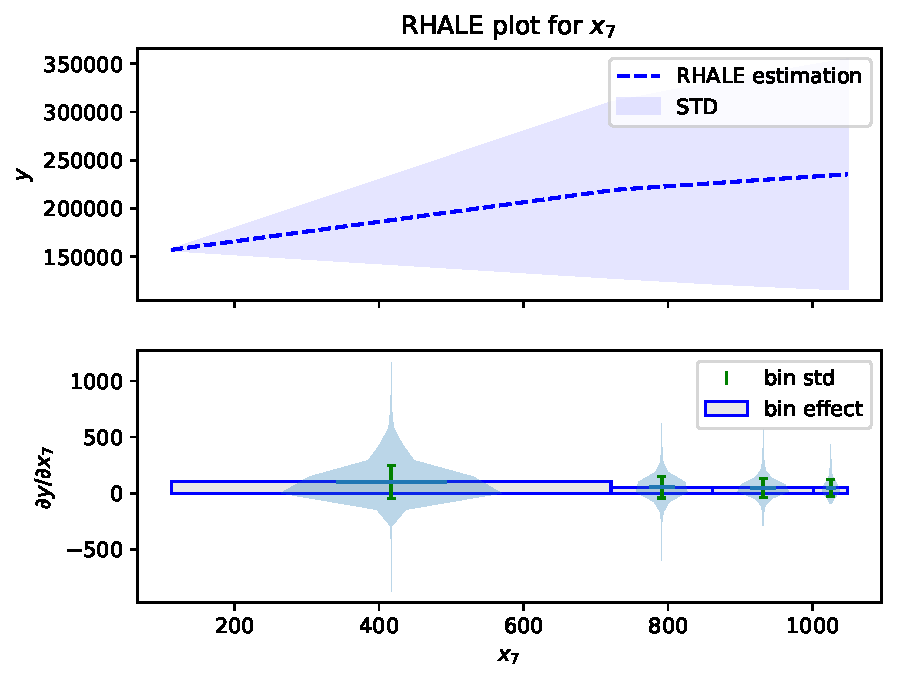
\includegraphics[width=.24\textwidth]{real_dataset_3/feature_6_ale_auto}
  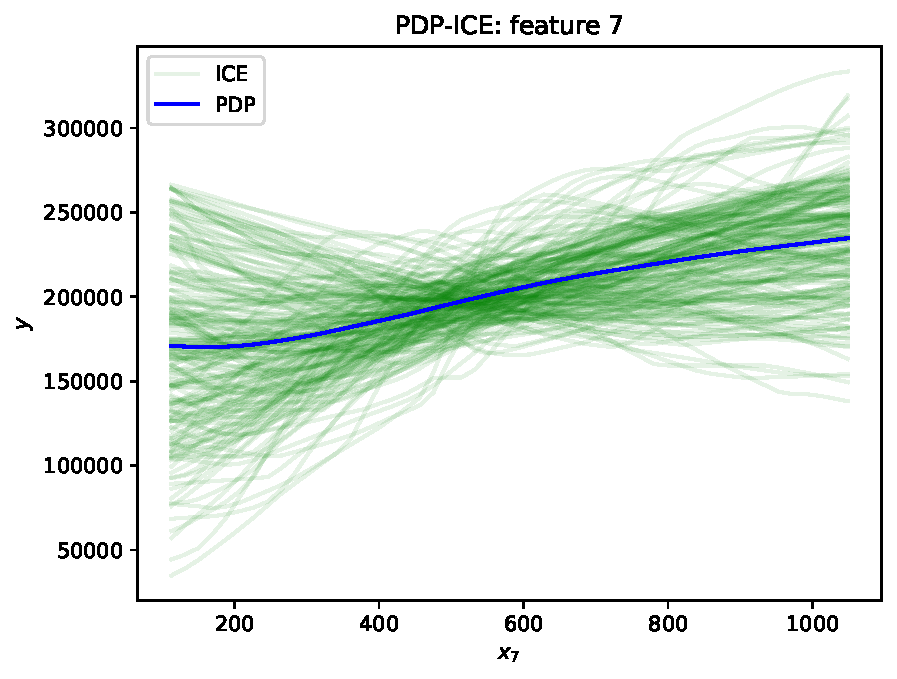
\includegraphics[width=.24\textwidth]{real_dataset_3/feature_6_pdp_ice}
  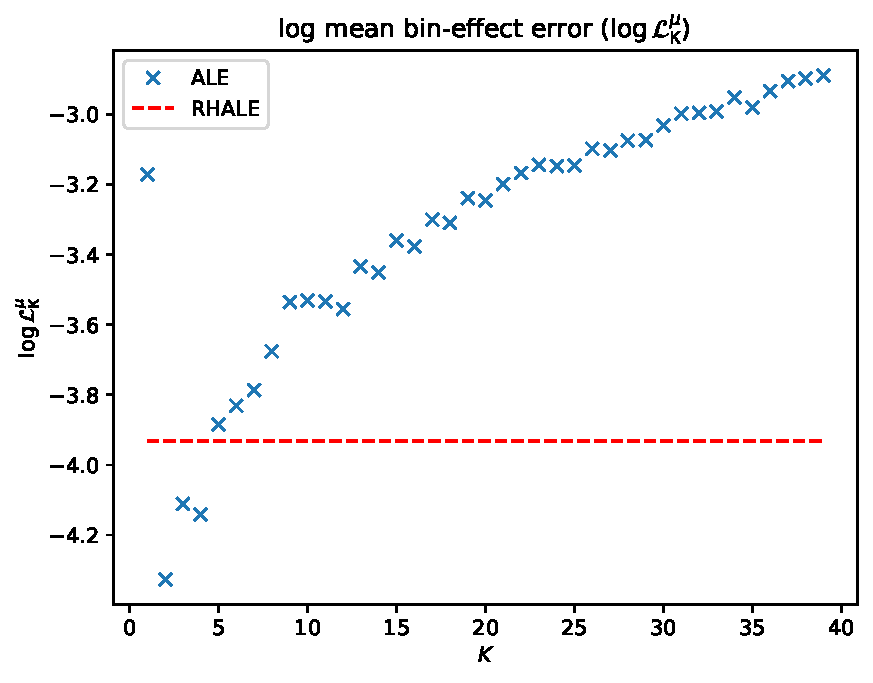
\includegraphics[width=.24\textwidth]{real_dataset_3/compare_mu_err_feature_6}
  \includegraphics[width=.24\textwidth]{real_dataset_3/compare_var_err_feature_6}\\
  \caption{From left to right: (a) RHALE plot, (b) PDP-ICE plot, (c) RHALE vs fixed-size \(\mathcal{L}^{\mu}\) and (d) RHALE vs fixed-size \(\mathcal{L}^{\sigma}\). From top to bottom, features \(x_1, x_3, x_4, x_5, x_7, x_8\).}
  \label{fig:ex-real-1-app}
\end{figure}


\bibliography{bibliography-supplement}

\end{document}
